\documentclass[12pt,a4paper]{report}
\usepackage{amsthm,amssymb,amsmath}
\usepackage[top=50mm, bottom=50mm, left=50mm, right=50mm]{geometry}

\usepackage{graphicx}
\usepackage{subcaption}
\usepackage[pagebackref=false,colorlinks,linkcolor=blue,citecolor=magenta]{hyperref}


\usepackage{geometry}
\usepackage{datetime} 
\usepackage{multirow}


\newcommand*{\BeginNoToc}{%
  \addtocontents{toc}{%
    \edef\protect\SavedTocDepth{\protect\the\protect\value{tocdepth}}%
  }%
  \addtocontents{toc}{%
    \protect\setcounter{tocdepth}{-10}%
  }%
}
\newcommand*{\EndNoToc}{%
  \addtocontents{toc}{%
    \protect\setcounter{tocdepth}{\protect\SavedTocDepth}%
  }%
}
\renewcommand{\bibname}{مراجع}
%\renewcommand{\refname}{مراجع}

%\usepackage[pagebackref=false]{hyperref}
\usepackage{tocbibind}
\usepackage{makeidx}
\makeindex
\usepackage{xepersian}
\settextfont[Scale=1.1]{B Nazanin}
% Latex 2020 2021 SetDigitFont error
\ExplSyntaxOn
\cs_set_eq:NN
\etex_iffontchar:D
\tex_iffontchar:D
\cs_undefine:N \c_one
\int_const:Nn \c_one { 1 }
\ExplSyntaxOff
\setdigitfont{Yas}
\defpersianfont\titr[Scale=1]{XB Titre}
\defpersianfont\nastaliq[Scale=1.5]{IranNastaliq}
\defpersianfont\traffic[Scale=1]{B Traffic}


\theoremstyle{definition}
\newtheorem{definition}{تعریف}[section]
\newtheorem{theorem}[definition]{قضیه}
\newtheorem{lemma}[definition]{لم}
\newtheorem{proposition}[definition]{گزاره}
\newtheorem{corollary}[definition]{نتیجه}
\newtheorem{remark}[definition]{ملاحظه}
\theoremstyle{definition}
\newtheorem{example}[definition]{مثال}


\begin{document}
	\newgeometry{total={210mm,297mm}, left=40mm, right=40mm, top=20mm, bottom=20mm,}
	\pagenumbering{harfi}
	\thispagestyle{empty}
	\vspace*{25mm}
	\centerline{
\includegraphics[height=4cm]{./images/logos/iust.png}}

	\begin{center}
	\textbf{
		دانشکده مهندسی کامپیوتر
	}
	\\[1cm]
	\baselineskip=2cm
	{\titr
	\begin{Huge}
	تشخیص ناهنجاری با استفاده از یادگیری عمیق\\[1cm]
	\end{Huge}}
	{\Large 
		\textbf{
			گزارش سمینار کارشناسی ارشد\\
			در رشته مهندسی کامپیوتر-گرایش هوش مصنوعی و رباتیک
		} \\[1cm]
	}

	{\Large { 
	نام دانشجو:
	}
	\\
	{\Large  علی نادری پاریزی }
	\\[.5cm]
	{\Large  
		استاد راهنما:
	}
	\\
	{\Large دکتر محسن سریانی}
	\\[.6cm]
	}
	اردیبهشت ماه ۱۴۰۱
	\end{center}

	\newpage
		\begin{center}
		
\includegraphics[width=\linewidth]{./images/god.png}
		\end{center}
	\newpage
	
	\newgeometry{total={210mm,297mm}, left=20mm, right=20mm, top=20mm, bottom=20mm,}
	
	\chapter*{چکیده}
	تشخیص ناهنجاری‌ مسئله مهمی است که در زمینه‌های تحقیقاتی گوناگون مورد مطالعه قرار می‌گیرد و کاربرد‌های بسیار زیادی دارد. یک نیاز مرسوم در حوزه تجزیه و تحلیل داده‌های دنیای واقعی، پی بردن به این است که بدانیم کدام نمونه‌ها از نقطه نظر تشابه رفتار و ظاهر با اکثریت نمونه‌های موجود بسیار متفاوت هستند. این تفاوت می‌تواند به دلیل خطای انداز‌ه‌گیری در هنگام جمع آوری داده‌ها باشد. گاهی اوقات این تفاوت می‌توانند نشان‌ دهنده وجود پدیده‌ای ناشناخته‌ باشد که در پشت‌پرده جامعه آماری مورد مطاالعه در حال رخ دادن است و ما از آن بی‌خبر هستیم. \\

در علم داده اصطلاح ناهنجاری به داده‌ای تعلق می‌گیرد از نقطه‌نظر یک معیار تشابه تعریف شده، میزان تشابه آن با سایر دادگان موجود بسیار کم باشد. برای مثال اگر عکس رادیولوژی فردی که بیماری ریوی دارد را با عکس‌های رادیولوژی گرفته شده از ریه افراد سالم مقایسه کنیم متوجه تفاوت این عکس با سایر عکس‌ها خواهیم شد. این عدم تشابه در دادگان، مشخص می‌کند  که فرد دچار بیماری ریوی است. درواقع پزشکان با مشاهده این عدم شباهت‌ها به وجود بیماری پی می‌برند. عمل مقایسه دادگان می‌تواند به وسیله کامپیوتر نیز انجام شود که موضوع این سمینار است.\\

در این سمینار تلاش شده روش‌های مبتنی بر یادگیری عمیق برای تشخیص ناهنجاری را برسی کنیم. از آنجا که کاربرد این موضوع در حوزه‌های گوناگون بسیار وسیع است و مقالات بسیار متعددی در رابطه با کاربردی‌های مختلف به چاپ رسیده، سعی کردیم حوزه سمینار را محدود کرده و ضمن معرفی انواع کاربرد‌های مسئله تشخیص ناهنجاری، به بررسی روش‌هایی بپردازیم که در رابطه با کاربرد پردازش تصویر و بینایی کامپیوتر هستند. با توجه به تعدد مقالات در سال‌های اخیر و وجود مقالات جامع در این حوزه، بیشتر مقالات جدید که در سال‌های اخیر منتشر شده‌اند را بررسی کنیم و برای باقی روش‌ها به ارجاع دهی به مقالات دیگر اکتفا کنیم.\\

	\textit{
واژه‌های کلیدی:
	}
	تشخیص ناهنجاری، پردازش تصویر، شبکه‌های عمیق

	\newpage
	\baselineskip=1cm
	\BeginNoToc
	\tableofcontents
	\listoffigures
	\listoftables
	\EndNoToc
	
	\newpage
	
	\baselineskip=.75cm
	\pagenumbering{arabic}
	%-------------------Chapter 1-----------------
	\chapter{مقدمه}
	تشخیص ناهنجاری‌\LTRfootnote{\lr{Anomaly detection}} مسئله مهمی است که در زمینه‌های تحقیقاتی گوناگون مورد مطالعه قرار می‌گیرد و کاربرد‌های بسیار زیادی دارد. یک نیاز مرسوم در حوزه تجزیه و تحلیل داده‌های دنیای واقعی، پی بردن این است که بدانیم کدام نمونه‌ها از نقطه نظر تشابه رفتار و ظاهر با اکثریت نمونه‌های موجود بسیار متفاوت هستند. این تفاوت می‌تواند به دلیل خطای انداز‌ه‌گیری در هنگام جمع آوری داده‌ها باشد. گاهی اوقات این تفاوت می‌توانند نشان‌ دهنده وجود پدیده‌ای ناشناخته‌ باشد که در پشت‌پرده جامعه آماری مورد مطاالعه در حال رخ دادن است و ما از آن بی‌خبر هستیم. 
	
	\begin{figure}[hp]
		  \begin{subfigure}{\linewidth}
			  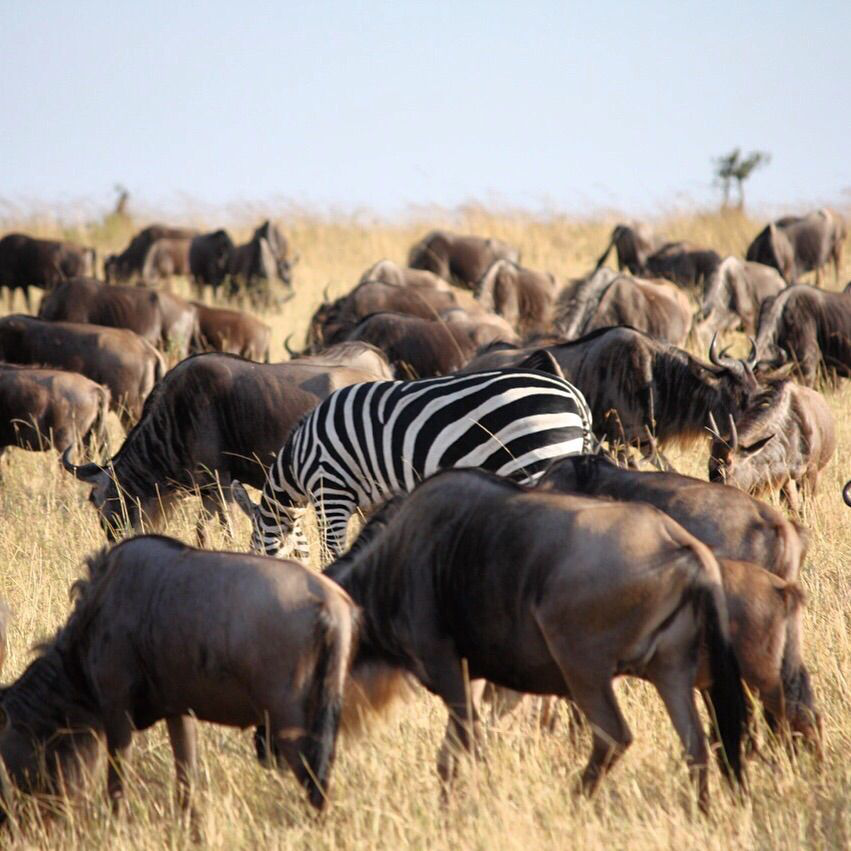
\includegraphics[width=.5\linewidth]{./images/figures/zibra-anomaly.png}\hfill
			  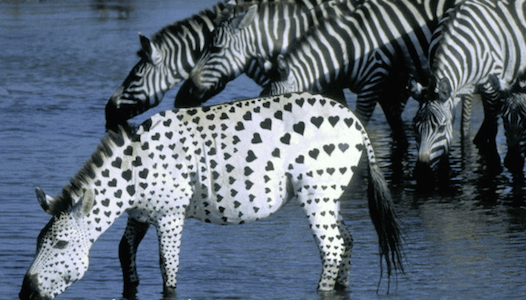
\includegraphics[width=.5\linewidth]{./images/figures/zibra-novel.png}
		  \end{subfigure}\par\medskip		  
		  \caption{مثالی از تفاوت دادگان ناهنجار و نوین}
		  \label{fig:novel-vs-anomaly}
	\end{figure}

در کنار ناهنجاری‌ها، دادگان دیگری نیز وجود دارند که با دادگان عادی متفاوت‌اند امّا این تفاوت به اندازی کافی زیاد نیست. به این دادگان اصطلاحا دادگان نوین\LTRfootnote{\lr{Novelties}} گفته می‌شود. دادگان نوین درواقع دادگانی هستند که در دسته دادگان عادی قرار می‌گیرند اما چون هنوز کشف نشده‌اند به نظر می‌رسد که با دادگان عادی تفاوت داشته باشند. برای مثال، اکثر ببر‌های دیده شده و شناخته شده به رنگ نارنجی و با خطوط راه راه سیاه هستند و دیدن بربر سفید برای ما تعجب آور خواهد بود. امّا همه به خوبی می‌دانیم که ببر سفید درواقع یک ببر است که فقط رنگ آن غیرعادی است و نباید آن را در دسته جدایی از حیوانات قرار داد.\\

در ادامه این فصل پس از تعریف ناهنجاری در دادگان، به بیان کاربرد‌های این بحث در حوزه‌های مختلف می‌پردازیم. سپس یک تعریف معیار که مرتبط با حوزه مورد نظر ما که همان پردازش تصویر است ارائه می‌دهیم. پس از تعریف حوزه مورد مطالعه و بررسی اهمیت موضوع، به توضیح ساختار کلی گزارش این سمینار خواهیم پرداخت.
		
	\section{مسئله تشخیص ناهنجاری}
تشخیص ناهنجاری که با عنوان تشخیص دادگان خارج از محدوده\LTRfootnote{Outlier detection} نیز شناخته می‌شود، به عملیاتی گفته می‌شود که طی آن به آشکارسازی نمونه‌هایی از مجموعه دادگان می‌پردازد که تفاوت زیادی با اکثریت دادگان موجود دارد. در واقع، اینجا تفاوت به معنی متفاوت بودن مشخصات و ویژگی‌های این نمونه‌ها با الگوی معمول موجود در مجموعه دادگان است. این مسئله یک موضوع فعال تحقیق در دهه‌های اخیر بوده که تقریبان از سال ۱۹۶۰ میلادی تا کنون مورد مطالعه قرار گرفته است~\cite{Grubbs1969ProceduresFD}. کاربردهای تشخیص ناهنجاری بسیار وسیع است و در حوزه‌های گوناگونی مورد استفاده قرار می‌گیرد.\\

ناهنجاری‌ها انواع مختلفی دارند که بسته به کاربرد و مفاهیم مختلف تعریف می‌شوند. به طور کلی می‌توان برای ناهنجاری‌ها سه نوع مختلف درنظر گرفت که عبارت اند از ناهنجاری نقطه‌ای\LTRfootnote{Point anomaly}،‌ ناهنجاری مفهومی‌\LTRfootnote{contextual anomalies}،‌ ناهنجاری مجموعه‌ای\LTRfootnote{collective anomalies}. اکثرکارهای انجام شده در متون علمی در مورد ناهنجاری نقطه‌ای بحث شده است. در این گونه ناهنجاری دادگان به صورت نقاطی در فضا درنظر گرفته می‌شوند و دادگان ناهنجار، نقاطی در فضای مورد نظر هستند که با دیگر دادگان فاصله دارند و رفتاری تصادفی از خود نشان می‌دهند که اغلب تفسیر خاصی ندارند. برا مثال مبلغ بسیار بالای تراکنش در یک رستوران  یک تراکنش غیر عادی به حساب می‌آید که با در نظر گرفتن آن در فضای بازنمایی دادگان این نقطه شباهتی به دیگر دادگان نخواهد داشت. دسته دوم ناهنجاری‌های مفهومی هستند که در این دسته مفهموم داده در یک مکان‌ و یا زمان‌ مختلف می‌تواند به صورت ناهنجاری درنظر گرفته شود. برای مثال عبور وسیله نقلیه در خیابان یک امر طبیعی است اما تردد وسایل نقلیه در مسیر عابرین پیاده یک پدیده غیرعادی است. نوع سوم ناهنجاری‌ها که اصطلاحا ناهنجاری مجموعه‌ای گفته می‌شود،‌مفهوم ناهنجاری از در یک سلسله از رویدادها دنبال می‌کند در حالی که هر رویداد یک داده کاملا عادی است. برای مثال در دنباله تراکنش‌های یک کارت اعتبار وجود چندین تراکنش یکسان با فواصل زمانی بسیار کم مشکوک است.

\begin{figure}[!hp]
	\begin{center}
		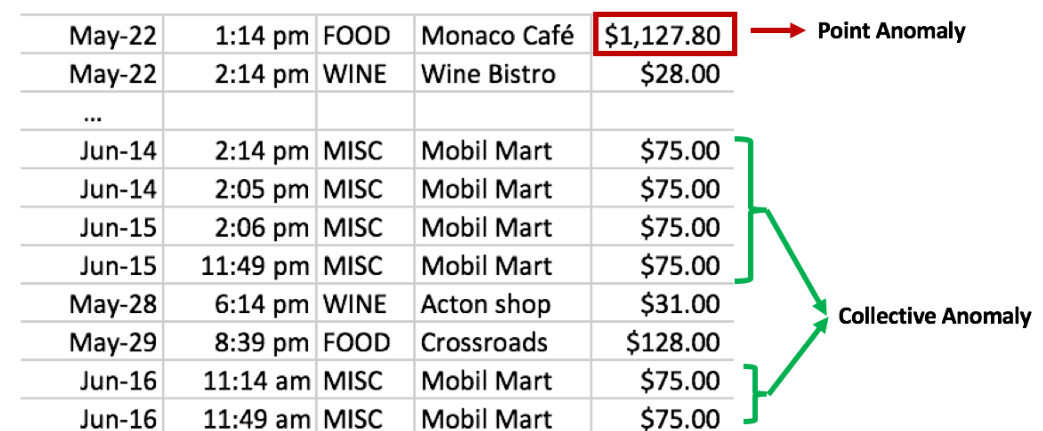
\includegraphics[width=0.7\linewidth]{./images/figures/credit-card.png}

		\caption{
		ناهنجاری نقطه‌ای و دنباله‌ای
		\cite{G.Chalapathy}
		}		
		\label{fig:anomaly-example-1}
		\centering
	\end{center}
\end{figure}

\section{جنبه‌های مختلف تشخیص ناهنجاری}
مسئله تشخیص ناهنجاری را جنبه‌های مختلفی می‌توان مورد بررسی قرار داد. برای مثال می‌توان روش‌های موجود را بر اساس ماهیت دادگان موجود مورد بررسی قرار داد و با توجه به نوع داده انواع روش‌ها را دسته‌بندی کرد. برای نمونه می‌توان ماهیت دادگان را به دودسته کلی، دنباله‌ای (مانند صدا، موسیقی، فیلم، متن و ...) غیر دنباله‌ای (مانند عکس، مشخصات بیمار و ...) تقسیم کرد. و یا بر اساس تعداد ویژگی‌های داده ورودی به دو دسته ابعاد پایین و ابعاد بالا تقسیم کرد. همچنین می‌توان روش‌های تشخیص ناهنجاری‌ها را از دید در دسترس بود برچسب دادگان مورد استفاده بررسی کرد. اما باید توجه داشت که پدیده‌های ناهنجار اصولا کم اتفاق می‌افتند و تعداد آنها در دادگان موجود کم است. با این حال می‌توان روش‌های تشخیص ناهنجاری را از دید رویکرد بر اساس در دسترس بودن برچسب دادگان به سه دسته باناظر، با نظارت ضعیف و همچنین بدون ناظر تقسیم کرد.

\section {کاربرد‌های مسئله تشخیص ناهنجاری}
برای درک اهمیت و کاربرد مسئله تشخیص ناهنجاری می‌توان به حجم مقالات چاپ شده در این حوزه و دامنه وسیع موضوعات تحقیقاتی اشاره کرد که حول این موضوع انجام شده و یا در حال انجام است. در این قسمت برخی از کاربرد‌های مسئله تشخیص ناهنجاری را به تفکیک حوزه‌های کاربردی مختلف می‌آوریم.

\subsection{امنیت سیستم و تشخیص نفوذ}
تشخیص نفوذ در کاربرد امنیت سایبری که عمل تشخیص و اطلاع پیدا کردن از دسترسی‌های غیر مجاز به شبکه و یا سامانه‌های رایانه‌ای است می‌تواند یکی از کاربرد‌های مسئله تشخیص ناهنجاری باشد. در اینگونه مسائل با بررسی گزارش‌های سیستم در طول زمان به عنوان داده ورودی به بررسی این قضیه می‌پردازند. همانطور که مشخص است، نوع  ناهنجاری در این جا میتواند از دو نوع دنباله‌ای و یا مفهومی باشد.

\subsection{تشخیص جعل اسناد و کلاهبرداری}
تشخیص مدارک جعلی در حوزه‌های مختلف مانند هویتی، بانکی، بیمه، کارت اعتباری و غیره بسیار کارآمد است. در اینگونه کاربردها نیز مدارک از جنبه‌های مختلفی با یکدیگر مقایسه می‌شوند تا مدارک جعلی از مدارک حقیقی تشخیص داده شوند. برای مثال، در جعل تراکنش‌های بانکی، میتوان با بررسی تاریخچه تراکنش‌ها، به عنوان داده ورودی، به یافتن تراکنش‌های غیر مجاز و جعلی پرداخت.

\subsection{سلامت و پزشکی}
بررسی گزارش‌های پزشکی یک حوزه بسیار فعال در علم کامپیوتر و مهندسی پزشکی بوده است. مقایسه و بررسی این گزارش‌ها از دید مسئله تشخیص ناهنجاری نیز بسیار مورد مطالعه قرار گرفته و کاربرد‌های فراوانی دارد. برای مثال در بررسی تصاویر پزشکی می‌توان از دید مسئله تشخیص ناهنجاری به یافتن بیماری‌ها و نواقص بیمار و علت بیماری پرداخت. همچنین بررسی 
گزارش علائم بیمار مانند ظربان قلب، سیگنال‌های مغز، فشار خون و غیره توسط دستگاه‌های پزشکی با هدف آگاهی از شرایط بحرانی و کنترل شرایط بیمار بسیار مناسب است. در این نوع کاربرد‌ها دادگان به صورت دنباله‌ای از رویداد‌ها به عنوان داده ورودی مورد بررسی قرار می‌گیرند تا در صورت بروز علائم و شرایط حیاطی غیر طبیعی از پیش‌آمدن اتفاقات ناگوار جلوگیری کنند.
\subsection{سامانه‌های هوشمد و اینترنت اشیا}
در سیستم‌های خانه هوشمند، سامانه‌های خودکار و اینترنت اشیا معمولا بسیاری از حسگر‌ها و دستگاه‌ها با استفاده از شبکه‌هایی به هم متصل شده‌اند که برای بررسی وضعیت کلی سیستم و اطمینان از کارکرد صحیح سیستم می‌توان رویداد‌های سامانه را در طول زمان مورد بررسی و ارزیابی قرار داد. کاربرد مسئله تشخیص ناهنجاری در اینجا بررسی گزارش‌های سامانه در طی زمان برای پی‌بردن به اتفاق افتادن شرایط نامتعادل و خطا‌های سامانه است.
\subsection{نظارت ویدیویی و سیستم‌های امنیتی}
دوربین‌های امنیتی در بسیاری از مکان‌ها برای بالابردن امنیت و همچنین نظارت بر افراد و وضعیت کلی مکان مورد استفاده قرار می‌گیرند اما بررسی و نظارت بر فیلم‌های ظبط شده توسط این دوربین‌ها کار بسیار دشوان و وقتی‌گیری است که در مقیاس وسیع این امر نزدیک به غیر ممکن می‌شود. برای مثال نظارت کار‌آمد دوربین‌های موجود در سطح شهر تهران برای کنترل ترافیک کار بسیار دشواری است و در صورتی که بخواهیم این کار را با استفاده از منابع انسانی انجام دهیم کار وقت و منابع بسیاری را طلب می‌کند. یکی از کاربرد‌های مسئله تشخیص ناهنجاری در این حوزه بررسی ویدیو‌ها و تلاش برای یافتن پدیده‌های غیر عادی است. برای مثال تشخیص ناهنجاری در تشخیص عبور غیرمجاز وسایل نقلیه، تشخیص تخلف‌های رانندگی، بررسی امنیت مکان‌های عمومی، وضعیت خط تولید کارخانه برای یافتن کالاهای معیوب و کاربرد‌های دیگری از این قبیل بسیار مورد استفاده قرار می‌گیرد.
\begin{figure}[!hp]
	\begin{center}
		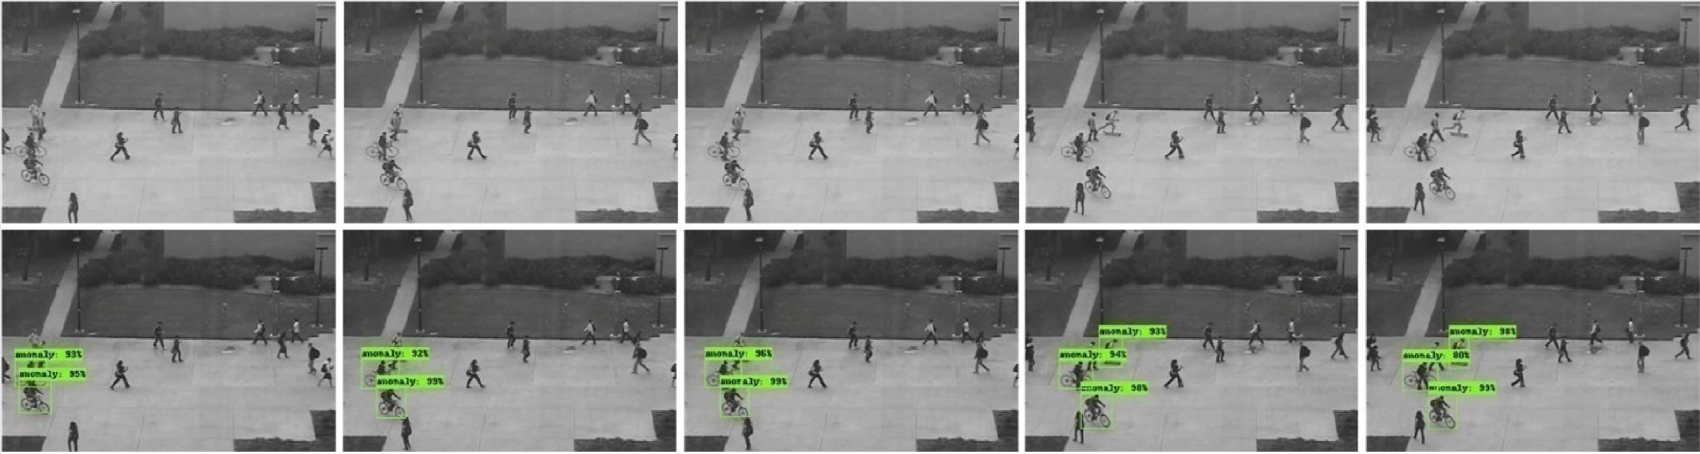
\includegraphics[width=\linewidth]{./images/figures/walkway-anomaly.png}
		\caption{ناهنجاری در کاربرد نظارت ویدیو~\cite{10.1016/j.compeleceng.2019.02.017}}
		\label{fig:walkway-anomaly}
	\end{center}
\end{figure}

\begin{figure}[!hp]
	\begin{center}
		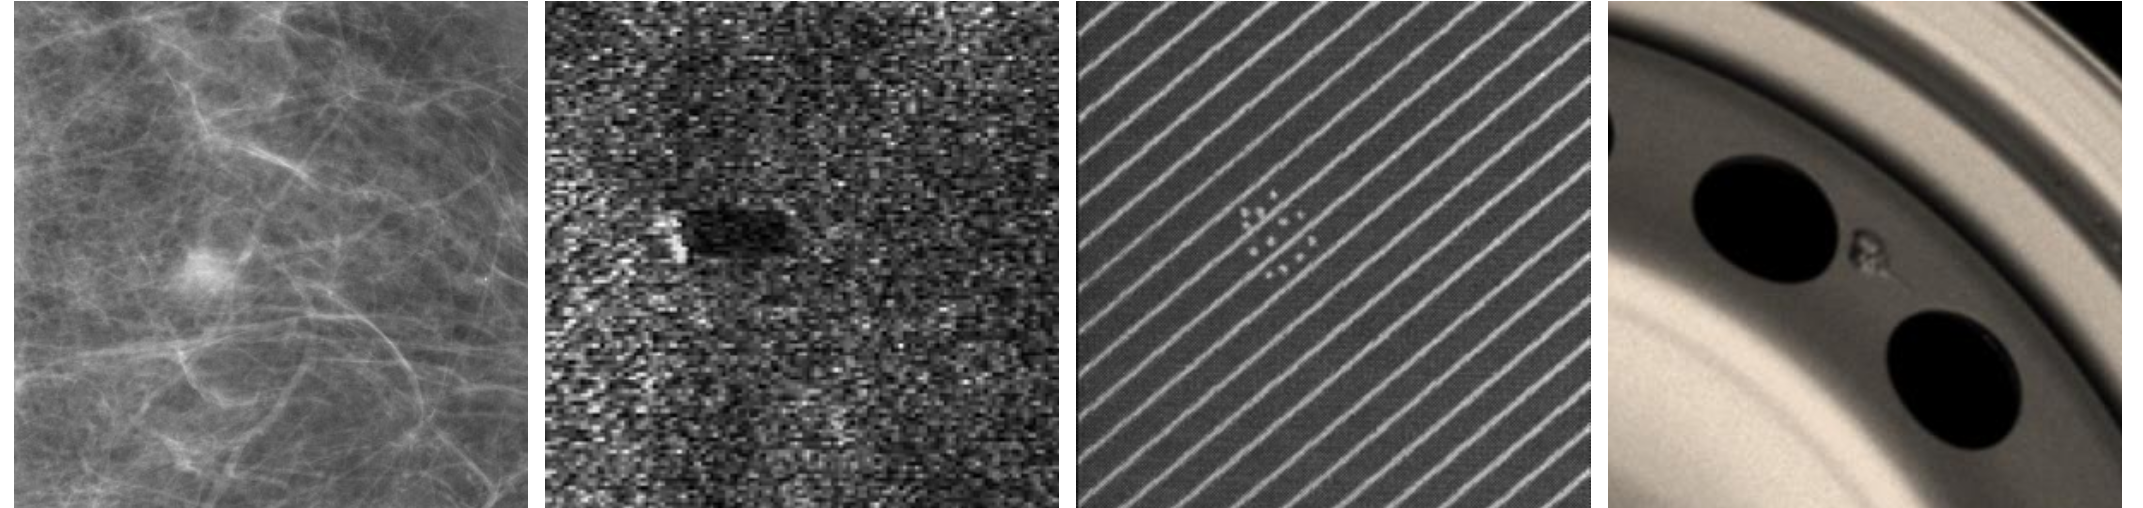
\includegraphics[width=\linewidth]{./images/figures/image-anomaly-examples-1.png}
		\caption*{به ترتیب از سمت چپ، توده سرطان سینه، مین زیر‌دریایی، نقص رنگ‌آمیزی کاشی تولید شده در کارخانه،نمونه نقص موجود در چرخ خودرو.}
		\caption{
		مثال‌هایی از ناهنجاری در تصاویر
		\cite{T.Ehret}
		}		
		\label{fig:anomaly-example-1}
		\centering
	\end{center}
\end{figure}

\subsection{خودرو‌های خودران}
یکی دیگر از حوزه‌های بسیار پرطرفدار در سال‌های اخیر ساخت خودرو‌های خودران و رانندگی خودکار وسایل نقلیه مختلف است. در این گونه سسیتم‌ها نیز می‌توان با بررسی وضعیت حسگر‌ها و دوربین‌های نصب شده بر روی وسیله نقلیه به بررسی خطرات احتمالی و شرایط غیرعادی مسیر درحال عبور پرداخت. با توجه به اینکه شرایط غیر عادی در رانندگی که منجر به تصادف و خطر شود به ندرت اتفاق می‌افتند و همچنین این شرایط می‌توانند به صورت‌ها و شکل‌ها مختلف روی دهند، استفاده از روش‌های تشخیص ناهنجاری در این کاربردها بسیار مورد پسند پژوهشگران این حوزه قرار گرفته است.


\section{ساختار کلی روش‌های تشخیص ناهنجاری}
	اگر بخواهیم روش‌های تشخیص ناهنجاری را به صورت عمومی توصیف کنیم، می‌توانیم بگوییم که این روش‌ها از سه بخش اصلی تشکیل شده‌اند. بخش اوّل یادگیری بازنمایی داد‌ه‌ها\LTRfootnote{Data representation} است. در این مرحله نگاشتی از دادگان ورودی به فضایی معیین آموخته می‌شود. این نگاشت را می‌توان به صورت تابعی مانند زیر تعریف کرد.
\begin{equation}
f(.;\theta): x \rightarrow y
\end{equation}
	
در بخش دوّم به تعریف یک معیار سنجش پرداخته می‌شود که برای ارزیابی خروجی مرحله قبل استفاده می‌شود. این معیار با دریافت خروجی مرحله اوّل یک امتیاز برای سنجش میزان تعلق داده ورودی به دسته ناهنجار اختصاص می‌دهد که به آن امتیاز ناهنجاری\LTRfootnote{Anomaly score} گوییم.
\begin{equation}
d(f(x);\eta): f(x) \rightarrow d \  ,\  d \in \mathbb{R}
\end{equation}

در آخر نیز با درنظر گرفتن یک مقدار آستانه $\delta$، به تصمیم‌گیری در مورد داده ورودی با توجه به امتیاز اختصاص داده شده در مرحله دوّم پرداخته می‌شود.

$$
\left\{
	\begin{array}{ll}
		anomaly  & d \geq \delta \\
		not\ anomaly & d < \delta
	\end{array}
\right.
$$

با توجه به این تعریف، رویکرد‌های موجود می‌توانند انواع زیر را داشته باشند:
\begin{enumerate}
	\item {غیر پارامتری: نیازی به یادگیری $\theta$ و $\eta$ و $\delta$ نیست.}
	\item{یک مرحله‌ای: تنها یکی از مجموعه پارامترهای موجود $\theta$ یا  $\eta$ یاد‌گرفته می‌شوند.}
	\item{دو مرحله‌ای:‌ هر دو مجموعه پارامتر $\theta$ و $\eta$ به صورت مستقل و جداگانه یاد‌گرفته می‌شوند.}
	\item{ادغامی\LTRfootnote{Integrated}: هر دو مجموعه پارامتر $\theta$ و $\eta$ باهم یادگرفته می‌شوند. }
\end{enumerate}

درصورت عدم وجود برچسب‌های دادگان موجود، ناچار به استفاده از روش بدون ناظر هستیم که در آن از هیچ گونه اطلاعاتی در مورد ماهیت دادگان استفاده نمی‌شود. در  این گونه مواقع معمولا $\delta$ از پیش تعریف شده است و یا همراه با  $\eta$ یادگرفته می‌شود. در حالتی که تنها بخشی از دادگان برچسب خورده باشند و باقی برچسب نخورده، می‌توانیم از رویکرد یادگیری با نظارت ضعیف استفاده کرد. در این مورد نیز مقدار آستانه می‌تواند با استفاده از تنظیم دقیق مدل بدست آید.
	
	\section{ساختار گزارش}
در فصل اوّل این سمینار به معرفی حوزه سمینار و تعریف مسئله پرداخته شد و در فصل دوّم به بررسی کلی روش‌ها سنتی در مسئله تشخیص ناهنجاری خواهیم پرداخت. فصل سوّم نیز در رابطه با بررسی روش‌های عمیق مورد استفاده در مقالات روز و معرفی کار‌های مرتبط با این سمینار و بررسی جزئی از روش‌ها و مقالات موجود چاپ شده در سال‌های اخیر خواهد خواهد بود. در فصل سوّم پس از معرفی هر یک از روش‌ها، چند نمونه مقاله به روز و مرتبط با آن دسته معرفی می‌شوند. در نهایت، در فصل چهارم، مسائل باز و کار‌های آینده این حوزه معرفی شده و چند نمونه پیشنهاد برای پروژه نهایی مطرح می‌شود.
	%------------Chapter 2--------------
	\chapter{مروری بر روش‌های سنتی}
	اگر به‌ یاد داشته باشید، در ابتدای فصل یک به این نکته اشاره شد که مسئله تشخیص ناهنجاری، یک موضوع فعال تحقیق در چند دهه اخیر است که یکی از مقالات معتبر چاپ شده آن مربوط به دهه ۱۹۶۰ میلادی می‌شود. از این رو، در طی این مدت بسیاری از روش‌ها برای یافتن دادگان خارج از محدوده معرفی و توسعه داده شده‌اند که از یادگیری عمیق استفاده نمی‌کنند. این روش‌ها به صورت عمده دادگان را مجموعه‌ای از نقاط در یک فضای چند بعدی فرض می‌کنند و تلاش آنها برای این است که نقاط خارج از محدوده را در این فضا با توجه به ویژگی‌ها و مشخصات دیگر نقاط آشکار کنند. عمدتاً این اینگونه روش‌ها را می‌توان از نقطه‌نظر ایده اصلی به سه دسته کلی استفاده از رده‌بندی، معیار فاصله و مدل‌های آماری تقسیم کرد\footnote{ر.ک جدول~\ref{table:traditional-category}}. در ادامه به مرور کلی این روش‌ها خواهیم پرداخت. با توجه به اینکه تمرکز ما بر بررسی کامل این روش‌ها نیست پیشنهاد می‌شود برای آشنایی بیشتر با این‌گونه روش‌ها به مقاله چاندولا و همکاران مراجعه کنید~\cite{V.Chandola}.
	
\begin{center}
\begin{table}[!h]
\begin{tabular}{ |p{4cm}|p{4cm}|p{4cm}|p{4cm}| } 
\hline
\multicolumn{4}{|c|}{دسته‌بندی روش‌های سنتی در تشخیص ناهنجاری}  \\
\hline

رویکرد ‌ & خلاصه ایده & انواع & روش‌های شناخته شده \\
\hline
رده‌بندی & یادگیری یک مرز تفکیک میان دادگان عادی و ناهنجار & یک کلاسه & \latin{One-class SVM} \latin{SVDD} \\
\cline{3-4}
& & چند کلاسه & - \\

\hline
معیار فاصله & اقدام به تعریف یک معیار فاصله می‌کند تا دادگان عادی را از دادگان ناهنجار جدا کند &  فاصله تا نزدیک ترین همسایه &  \latin{LOC}\LTRfootnote{Local Outlier Factor}  \latin{COF} \\
\cline{3-4}
&&خوشه بندی و سنجش فاصله تا نزدیک ترین خوشه& \latin{K-means} \latin{CBLOF} \\

\cline{3-4}
&&استفاده از تصویر سازی نقاط در فضایی با ابعاد کمتر& \latin{PCA} \latin{Isolation Forest} \\

\hline 
مدل آماری & دادگان عادی در نواحی پر احتمال مدل آماری قرار می‌گیرند & روش‌های پارامتری  & \latin{Gausian Mixture Model} \\
\cline{3-4}
&&روش‌های غیر پارامتری ‌& \latin{Kernel destiny estimator} \\
\hline

\end{tabular}
\caption{دسته‌بندی روش‌های سنتی}
\label{table:traditional-category}
\end{table}
\end{center}

\section{روش‌های مبتنی بر رده‌بندی}
همانطور که در ابتدای این بخش گفته شد، یکی از ایده‌های کلی در روش‌های مورد استفاده برای تشخیص ناهنجاری استفاده از ایده رده‌بندی است. در اینگونه روش‌ها تلاش می‌شود یک مرز تفکیک میان دادگان عادی و دادگان ناهنجار رسم شود. اگر چنین مرزی وجود داشته باشد، می‌توانیم با استفاده از الگوریتم‌های رده‌بند موجود اقدام به یافتن این مرز کرد و سپس با استفاده از مدل آموزش دیده اقدام به آشکارسازی داده‌های ناهنجار کرد. همانطور که مشخص است در این گونه روش‌ها تنها یک دسته برای دادگان تعریف می‌شود که آن دسته دادگان عادی است. دیگر دادگانی که در این دسته قرار نمی‌گیرند به عنوان دادگان عادی در نظر گرفته می‌شوند. البته استفاده از رویکرد رده‌بندی چند کلاسه نیز در صورت وجود برچسب برای تمامی دادگان امکان پذیر است امّا استفاده از این روش کمتر مرسوم است. یکی از معروف ترین روش‌های مورد استفاده دسته بند بردار پشتیبان یک کلاسه\LTRfootnote{One-class SVM} است.

در ماشین بردار پشتیبان ما به دنبال یافتن یک ابر صفحه جدا کننده میان دو دسته داده موجود هستیم. در الگوریتم بردار پشتیبان یک کلاسه ما درواقع به دنبال یافتن صفحه ای هستیم که دادگان معمول در یک طرف این صفحه قرار بگیرند. در این روش تلاش می‌شود صفحه مورد نظر تا حد امکان به نقاد داده نزدیک باشند. پس از رسم این صفحه، دادگانی که به مبدا مختصات نزدیک تر هستند در دسته ناهنجاری‌ها قرار می‌گیرند \cite{10.5555/3009657.3009740}.

در اینجا تابع نگاشتی که باید یاد کرفته شود همان تابع کرنل در ماشین بردار پشتیبان است و تابع امتیاز ناهنجاری نیز به صورت اندازه فاصله از مبدا مختصات تعریف می‌شود. شکل~\ref{fig:one-class-svm} این روش را به تصویر کشیده است. توجه داشته باشید که در اینجا تنها یک دسته برای رده‌بندی تعریف می‌شود که آن دسته دادگان عادی است، پس نیازی به وجود برچسب برای تمامی دادگان نیست و رویکرد ما در اینجا به صورت کاملا بدون ناظر خواهد بود.
\begin{figure}[!h]
	\begin{center}
		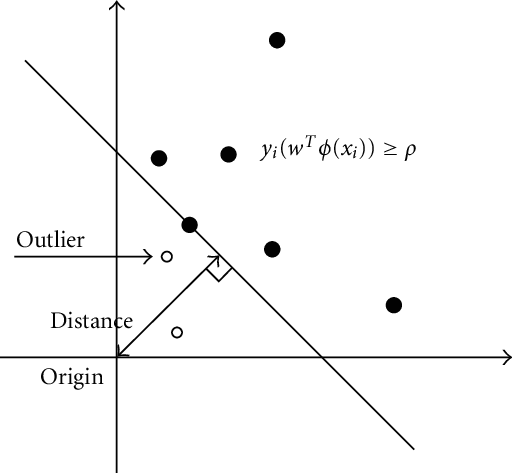
\includegraphics[width=0.5\linewidth]{./images/figures/one-class-svm.png}
	\end{center}
	\caption{ماشین بردار پشتیبان یک کلاسه}
	\label{fig:one-class-svm}
	\centering
\end{figure}


نمونه دیگری از روش‌های مورد استفاده برای آشکارسازی ناهنجاری که از رویکرد رده‌بندی استفاده می‌کند، بردار پتیبان توصیفگر داده‌\LTRfootnote{Support Vector Data Description (SVDD)} است. در این روش سعی می‌شود کره‌ای با کوچک ترین اندازه ممکن حول دادگان موجور رسم شود. پس از رسم این کره، دادگانی که در خارج از آن قرار می‌گیرند به عنوان داده ناهنجار شناخته خواهند شد~\cite{pmlr-v80-ruff18a} .
\begin{figure}[!h]
	\begin{center}
		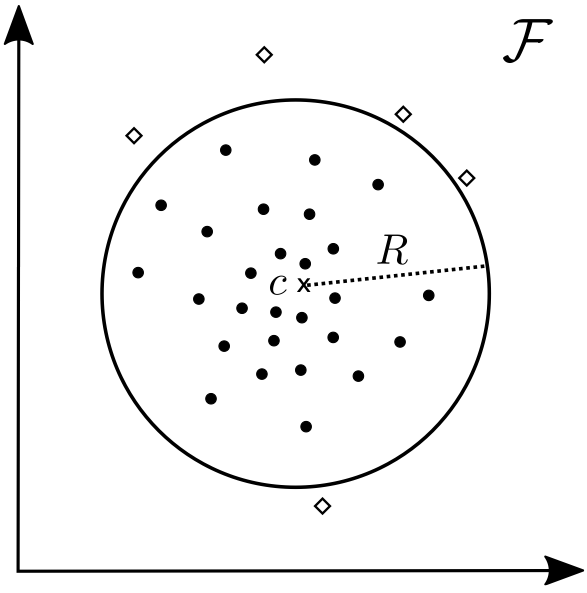
\includegraphics[width=0.5\linewidth]{./images/figures/svdd.png}
	\end{center}
	\caption{بردار پشتیبان توصیفگر داده عمیق~\cite{pmlr-v80-ruff18a}}
	\label{fig:deep-svdd}
	\centering
\end{figure}

ازجمله مزیت‌های این رویکرد،‌آموزش سریع، و دقت بهتر آن در مواقعی است که دادگان برچسب خورده در اختیار هستند. و از معایب این روش در هنگام استفاده از رده‌بندی چند کلاسه می‌توان به نیاز برای چندین دسته داده عادی یاد کرد. همچنین این رویکرد‌ها نیاز به تعیین ابرپارامتر برای مدل یادگیری دارند.

\section{روش‌های مبتنی بر معیار فاصله}
اگر به دادگان موجود را به صورت نقاطی بازنمایی شده بر روی صفحه مختصات نگاه کنیم،‌ می‌توانیم از معیار فاصله نقاط از یکدیگر به تصمیم‌گیری در مورد دادگان بپردازیم. در اینگونه رویکرد‌ها معمولا اقدام به تعریف یک معیار فاصله می‌کنند تا دادگان عادی را از دادگان ناهنجار جدا کنند. یک نمونه روش معروف که در این دسته می‌گنجد روش معروف عامل پرت محلی\LTRfootnote{Local Outlier Factor} است. در این روش میانگین فاصله هر نقطه از همسایگان محلی محاسبه شده و اگر این میانگین از یک مقدار آستانه بیشتر باشد،‌داده به عنوان داده ناهنجار شناخته می‌شود. برای سادگی کار، میانگین فاصله نقطه تا تمام همسایگان را بر میانگین فاصله میان همسایگان نقطه محاسبه شده و مقدار آستان برابر با عدد یک درنظر گرفته می‌شود~\cite{10.1145/342009.335388}. در استفاده از این روش نیز نیازی به وجود برچسب دادگان نیست همچنین این روش پارامتری برای یادگیری ندارد و در دسته روش‌های بدون پارامتر نیز قرار می‌گیرد. در واقع این گونه روش‌ها معمولا به صورت بدون ناظر هستند.


	\begin{figure}[!h]
	\begin{center}
		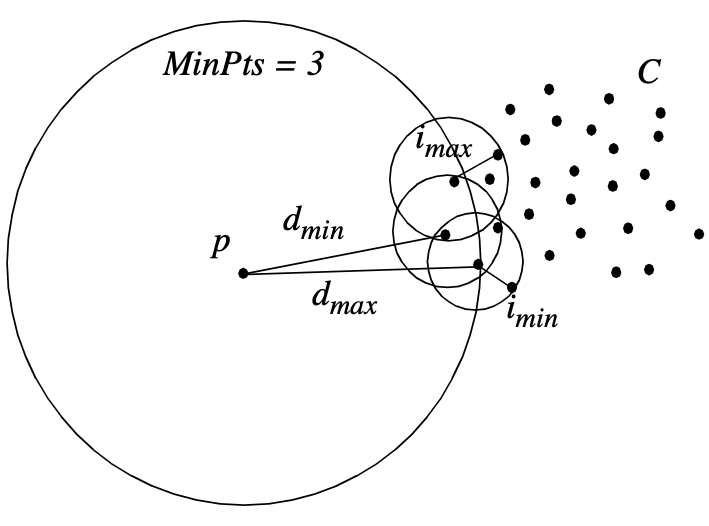
\includegraphics[width=0.5\linewidth]{./images/figures/lof.png}
	\end{center}
	\caption{نمایش کلی روش عامل پرت محلی~\cite{10.1145/342009.335388}}
	\label{fig:lof}
	\centering
\end{figure}



\section{روش‌های مبتنی بر مدل آماری}
ایده اصلی در این دسته از رویکرد‌ها بدین صورت است که، دادگان عادی همواره احتمال رخدادن بالایی دارند، در نتیجه در نواحی از مدل مدل آماری قرار می‌گیرند که احتمال وقوع آنها بیشتر است. برای مثال در روش مدل خطی پویا\LTRfootnote{Dynamic liner model} ابتدا دادگان را از فضای ورودی به یک فضای از پیش تعیین شده نگاشت می‌کنیم. سپس با استفاده از مدل بدست آمده سعی در پیشبینی مقدار ورودی با توجه به دیگر دادگان موجود می‌کنیم. در اینجا امتیاز ناهنجاری میزان تفاوت مقدار پیشبینی شده و مقدار حقیقی داده است. اگر مقدار اختلاف از یک مقدار آستانه از پیش تعیین شده، که با استفاده از آزمایش با دادگان برچسب خورده بدست آمده، بیشتر باشد، به دسته دادگان ناهنجار تعلق می‌گیرد.


	\chapter{روش‌های مبتنی بر یادگیری عمیق}
	در این فصل‌ ابتدا به معرفی مدل‌های پایه‌ای یادگیری عمیق خواهیم پرداخت که در تشخیص ناهنجاری مورد استفاده قرار می‌گیرند. ینگونه مدل‌ها، پایه و اساس خیلی از روش‌های ارائه شده هستند و آشنایی با آنها به درک بهتر مطلب کمک بسیار زیادی خواهد کرد. پس از معرفی ساختار مورد بحث نمونه‌هایی از کار‌های انجام شده که از آن استفاده می‌‎کنند را به اختصار معرفی خواهیم کرد. جدول~\ref{table:deep-structures} لیستی از روش‌های مورد بحث در این بخش را جمع آوری کرده است.

	
\begin{table}[!h]
	\begin{center}
			\begin{tabular}{ |c|c|c| } 
				\hline
				\multicolumn{3}{|c|}{مدل‌های پایه‌ مورد استفاده در روش‌های عمیق برای تشخیص ناهنجاری}  \\
				\hline
				
				نام مدل ‌ & مقاله مرجع & مزیت استفاده \\
				\hline
				\latin{AE} & & \\
				\hline
				\latin{SAE} & & \\
				\hline
				\latin{DAE} & & \\
				\hline
				\latin{RDA} & & \\
				\hline
				\latin{VAE} & & \\
				\hline
				\latin{ِDCAE} & & \\
				\hline					
				\latin{DTS} & & \\
				\hline
				\latin{GAN} & & \\
				\hline	
			
			\end{tabular}
			\caption{الگوریتم‌های عمیق مورد استفاده در تشخیص ناهنجاری}
			\label{table:deep-structures}
		\end{center}
\end{table}

	\section{استفاده از ساختار‌های عمیق}
یکی از ابتدایی ترین ایده‌هایی که در مورد استفاده از روش‌های سنتی موجود با توجه به معرفی و پیشرفت ساختار‌های عمیق به ذهن می‌رسد، استفاده از این ساختار‌ها در روش‌های سنتی است. ساختار‌های عمیق با توجه به قابلیت بالای یادگیری ترکیب‌های غیر خطی گوناگون، می‌توانند به عنوان تابع نگاشت دادگان در روش‌های سنتی استفاده شوند تا بتوانند بازنمایی بسیار بهتری از دادگان را برای انجام عملیات امتیازدهی و تشخیص ناهنجاری بدست آورند.
مدل پرسپترون چند لایه‌ای\LTRfootnote{Multilayer Perceptron} یکی از ابتدایی ترین و مهم‌ترین مدل‌هایی است که می‌توان آنرا نقطه شروعی بر تمام روش‌های عمیق موجود در حال حاضر دانست. این مدل درواقع شبکه‌ای از نورون‌های عصبی مصنوعی\LTRfootnote{Perceptron} است که لایه‌های آن صورت کاملا متصل با یکدیگر ارتباط دارند. این شبکه دارای حداقل سه لایه ورودی، مخفی و خروجی است که در آن به غیر از نورون‌های لایه ورودی، باقی نورون‌ها دارای تابع فعال سازی غیر خطی هستند. این مدل برای یادگیری بازنمایی غیر خطی دادگان ورودی معرفی شده و در بسیاری از روش‌های تشخیص ناهنجاری کاربرد دارد. برای مثال در روش بردار پشتیبان توصیفگر داده که در فصل دوم معرفی شد می‌توان بجای تابع $f(.;\theta)$ که مسئول نگاش دادگان به فضایی معین برای بدست آورد بازنمایی خوبی از دادگان است از یک شبکه عمیق مانند مدل پرسپترون چندلایه استفاده کرد. این مدل به دلیل توانایی یادگیری نگاشت غیر خطی دادگان می‌تواند بازنمایی بهتری از دادگان را برای مرحله دوم محاسبات که همان عمل امتیاز دهی به نقاط است بدست آورد. راف و همکاران با استفاده از این ایده، روش بردار پشتیبان توصیف‌گر داده عمیق را معرفی کردن که در مقایسه با روش‌های سنتی عملکرد بسیار بهتری را از خود نشان داده است~\cite{pmlr-v80-ruff18a}. این روش در مقایسه با برخی روش‌های عمیق نیز نتایج بسیار مطلوبی را دربر داشته است که در بخش مقایسه روش‌ها این نتایج آورده خواهند شد.

\begin{figure}[!h]
	\begin{center}
		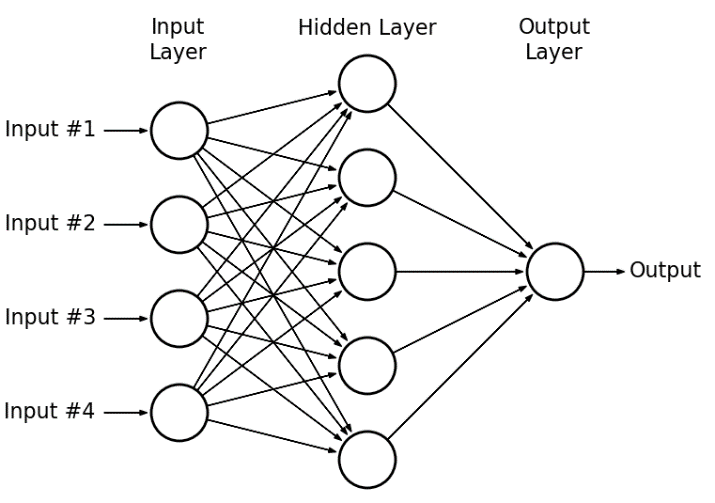
\includegraphics[width=0.5\linewidth]{./images/figures/mlp.png}
	\end{center}
	\caption{مدل پرسپترون چند لایه}
	\label{fig:mlp}
	\centering
\end{figure}

\begin{figure}[!h]
	\begin{center}
		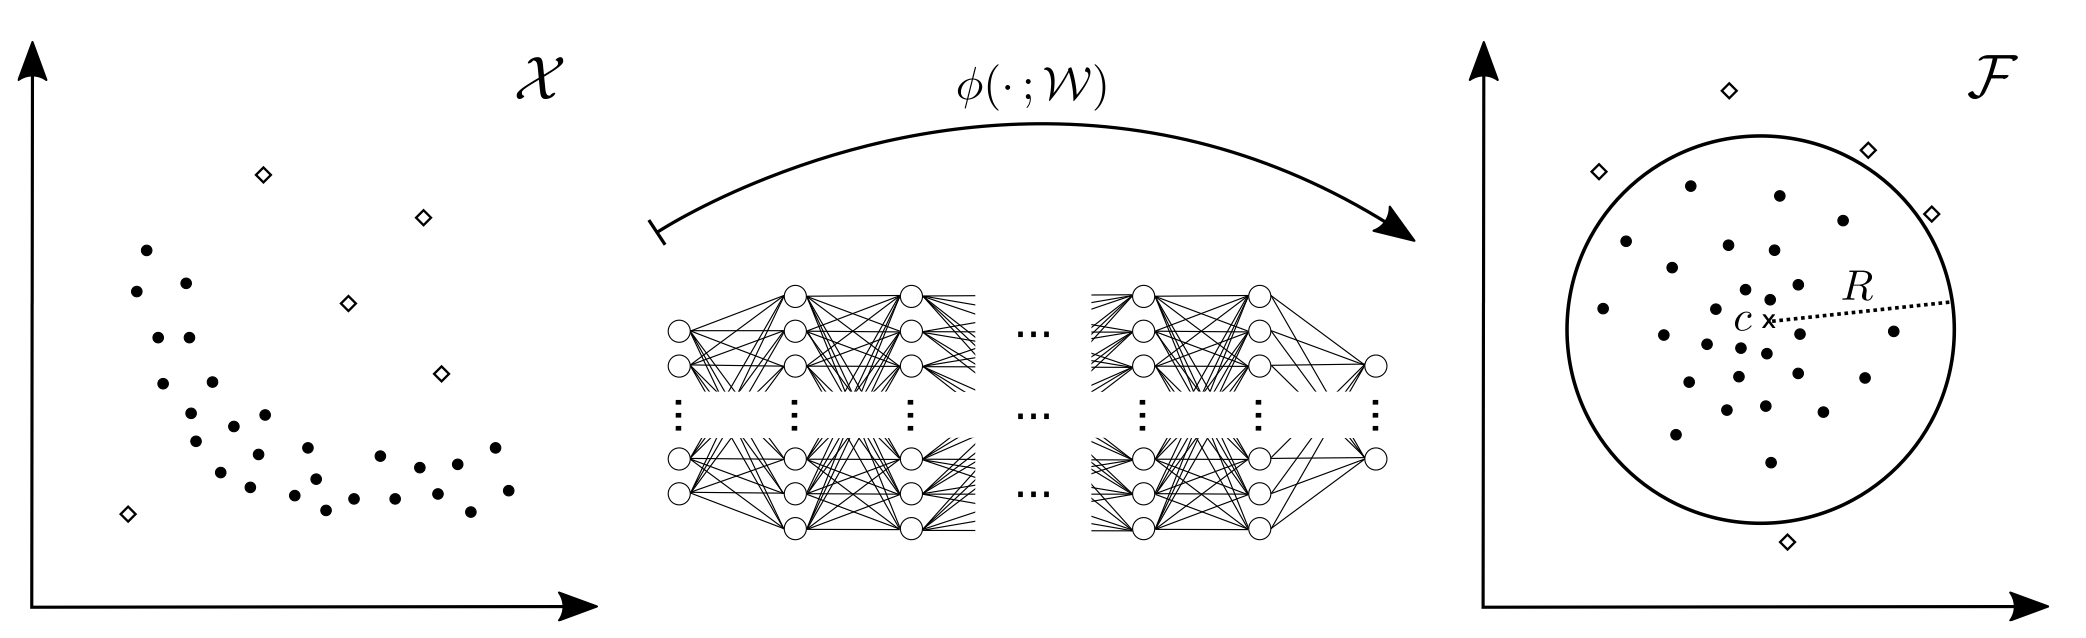
\includegraphics[width=\linewidth]{./images/figures/deep-svdd.png}
	\end{center}
	\caption{بردار پشتیبان توصیفگر داده عمیق~\cite{pmlr-v80-ruff18a}}
	\label{fig:deep-svdd}
	\centering
\end{figure}

	\section{خود رمزکننده}
	خودرمز کننده‌\LTRfootnote{AutoEncoder}ها نوعی از شبکه‌های عصبی هستند که از روش پس انتشار\LTRfootnote{Backpropagation} برای یادگیری ویژگی‌های مفهومی استفاده می‌کنند. این شبکه‌ها به صورت دو مرحله‌ای اقدام به یادگیری می‌کنند که به ترتیب رمزنگاری و رمزگشایی نام دارند. در مرحله اول داده ورودی به شبکه رمز کنند داده می‌شود و رمز کننده داده ورودی را به یک فضا با ابعاد پایین نگاشت می‌کند. به این فضا به اصطلاح فضای باقی‌مانده\LTRfootnote{Latent space} یا فضای $z$ می‌گویند. در مرحله دوم، بازنمایی بدست آمده وارد شبکه رمزگشا شده تا داده از فضای باقی مانده دوباره به فضای ورودی باز گردانده شود. آنچه که انتظار می‌رود آن است که خروجی مدل با آنچه در ورودی به مدل داده شده بسیار شبیه باشند. در این صورت قسمت رمز کنند توانسته بازنمایی خوبی از داده را در فضای باقی مانده ایجاد کند~\cite{BHUVANESHWARI2021131}.
\begin{figure}[!h]
	\begin{center}
		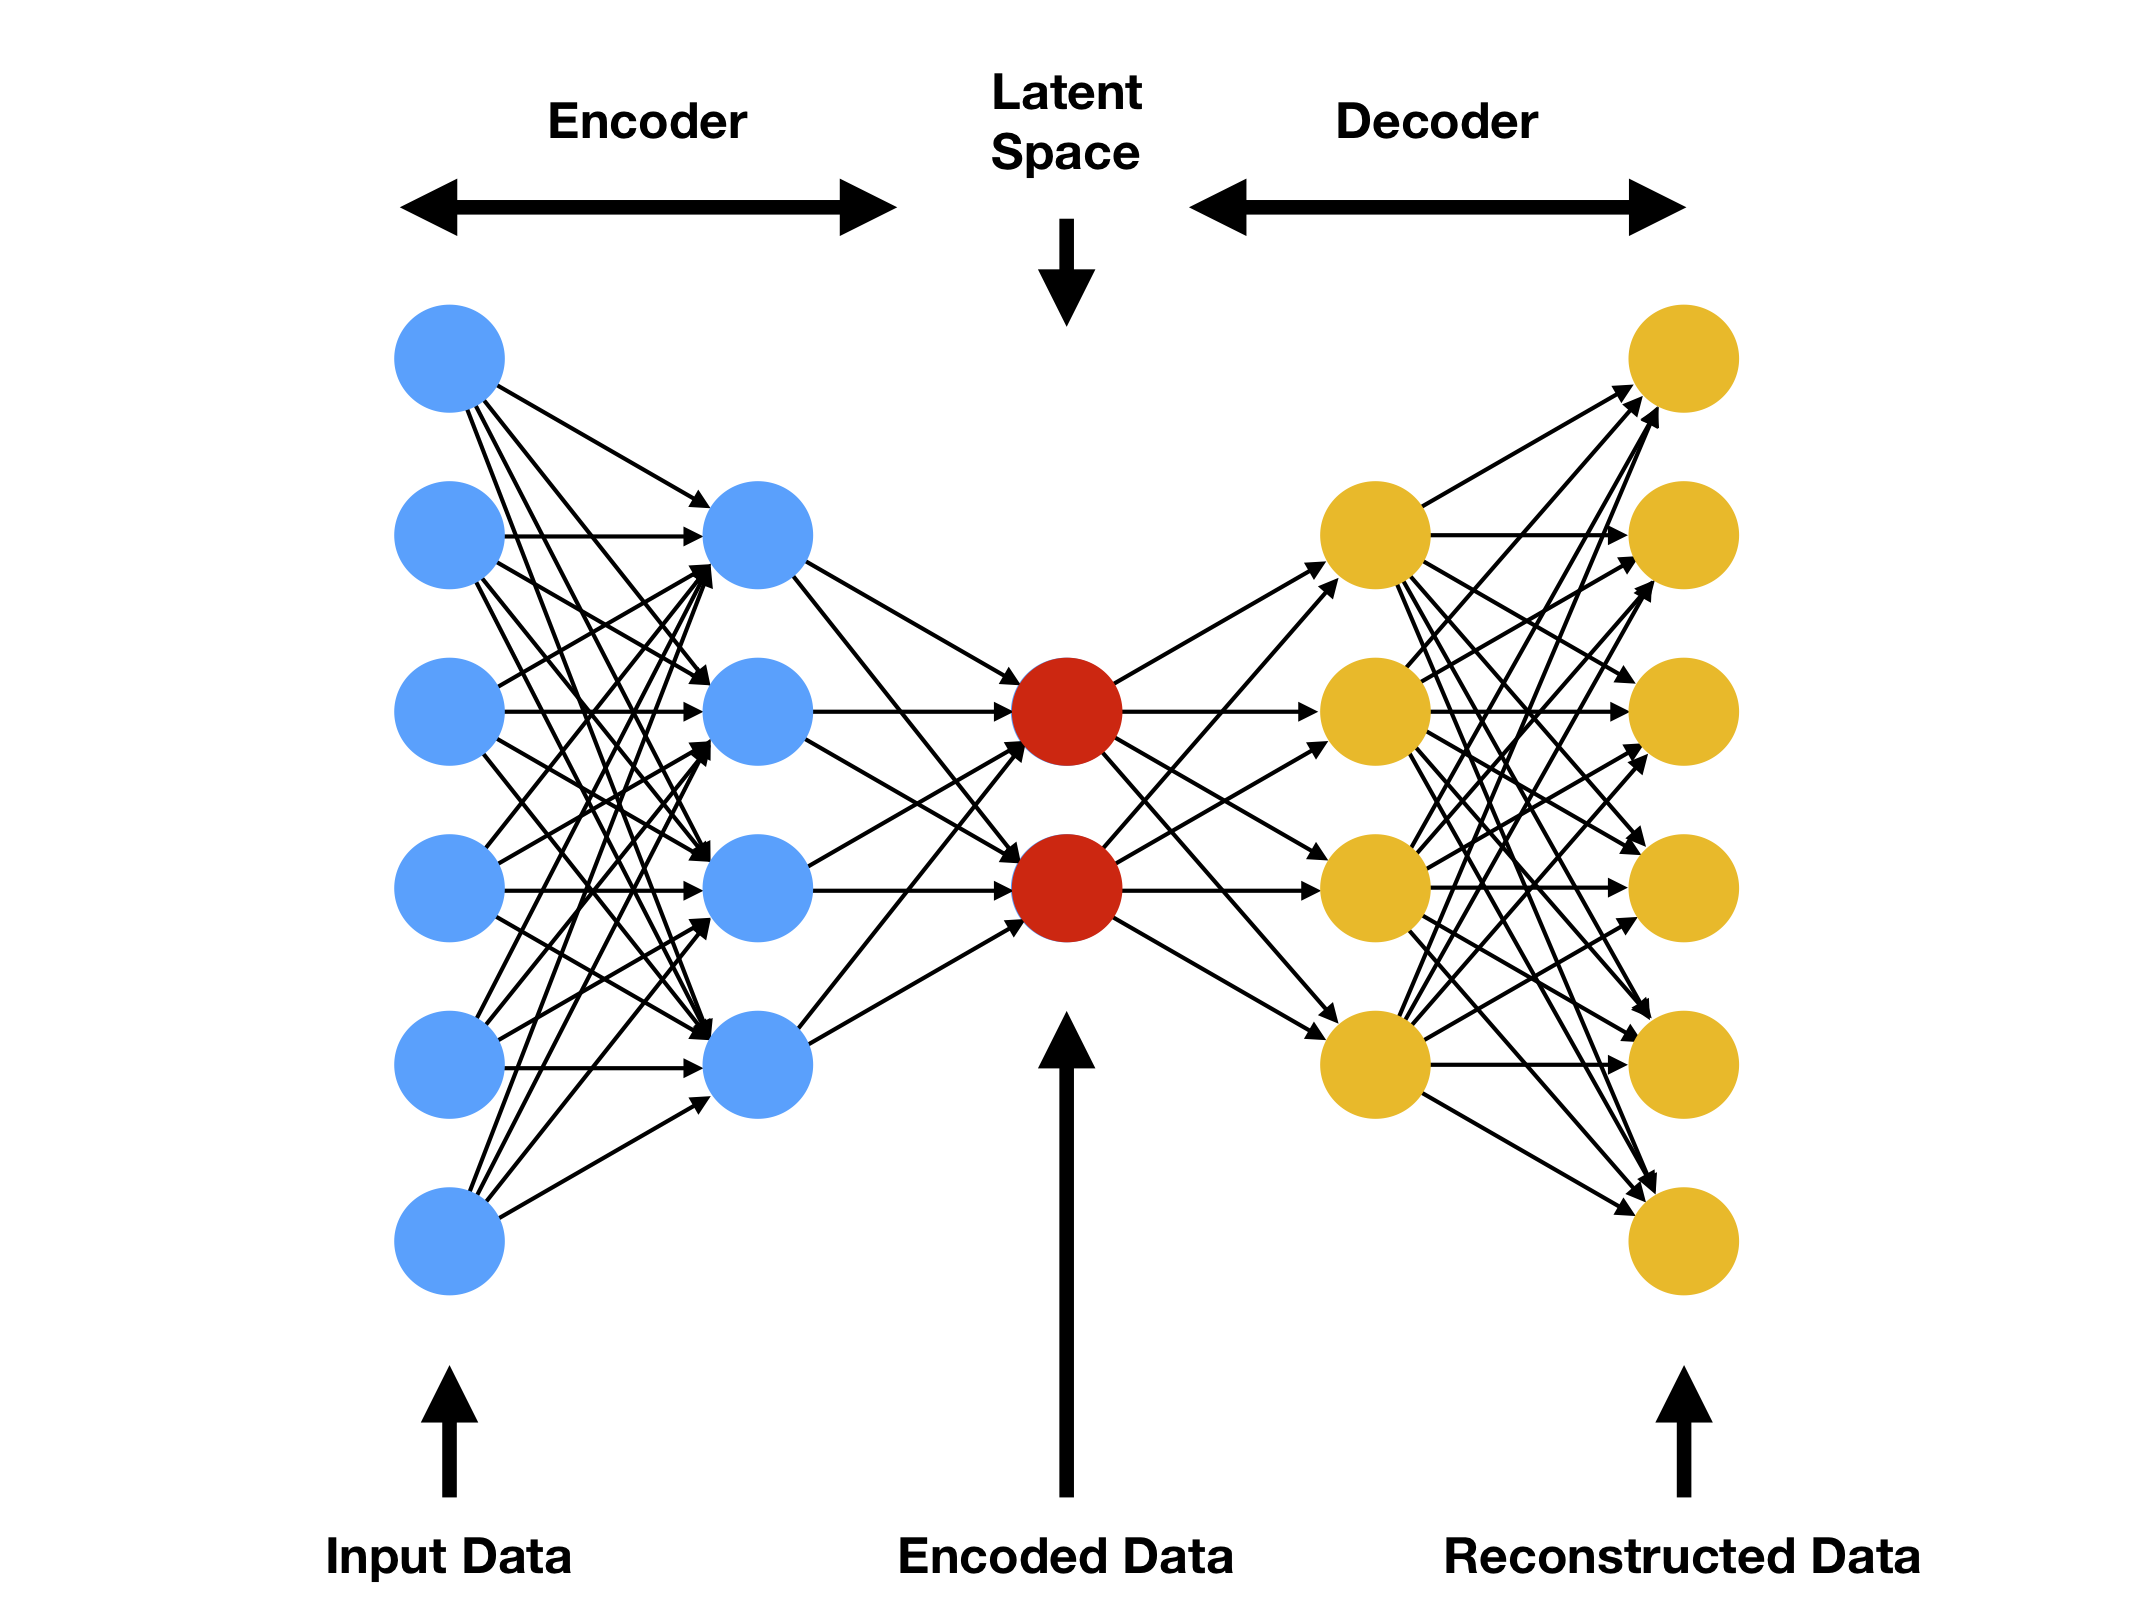
\includegraphics[width=0.6\linewidth]{./images/figures/ae.png}
	\end{center}
	\caption{مدل خود رمز کننده}
	\label{fig:ae}
	\centering
\end{figure}

اگر بخواهیم کارکرد مدل شکل~\ref{fig:ae} را با فرمول ریاضی توصیف کنیم، با در نظر داده $X$ به عنوان ورودی مدل، رمز کنند با گرفتن این ورودی، آن را به فضای باقی مانده و به نقطه $z$ نگاشت می‌کند. اگر تابع رمز کننده را $f$ بنامیم معادله مرحله اول به صورت زیر خواهد بود.
\begin{equation}
f(X, \theta_1): X \rightarrow z
\end{equation}
که در اینجا ابعاد فضای $z$ از ابعاد فضای ورودی $X$ کمتر است. این بدان معنی است که در اینجا عمل کاهش ابعاد ورودی صورت گرفته است. اگر رمزگشا را مانند تابعی درنظر بگیریم و آن‌را $g$ بنامیم، این تابع با دریافت ورودی $z$، اقدام به بازسازی داده ورودی می‌کند.
\begin{equation}
	g(z, \theta_2): z \rightarrow \hat{X}
\end{equation}

در کاربردهای تشخیص ناهنجاری معمولا در هنگام استفاه از این معماری، سعی می‌شود از تابع خطای مقایسه ورودی و خروجی مدل برای آموزش مدل استفاده کنند و در فرایند آموزش تنها از دادگان عادی استفاده شود. ایده اصلی در این گونه روش‌ها این است که با توجه به اینکه مدل تنها با دادگان عادی آموزش دیده است، دادگانی که توسط این مدل نتوانند به خوبی بازسازی شوند دارای ناهنجاری بوده‌اند. در واقع در اینجا تابع خطا که همان تابع امتیاز ناهنجاری است به صورت زیر تعریف می‌شود.
\begin{equation}
	L(X, g(f(x))) = d
\end{equation}

پس از آموزش مدل مقدار آستانه $\delta$ برای بدست آوردن بهترین نتیجه با آزمون و خطا و یا روش‌های دیگر مانند استفاده از نمودار حساسیت و دقت تعیین می‌شود. \\

خودرمز کننده‌ها باید به تغییرات دادگان ورودی حساس باشند تا بتوانند با دقت مطلوب داده رمز شده را بازسازی کنند. همچنین این حساسیت نباید به اندازه‌ای باشد که باعث بشود مدل بجای یادگیری عملکرد مناسب، به بخاطر سپاری دادگان ورودی بپردازد و دچار بیش‌برازش\LTRfootnote{Overfit} بشود. برای دستیابی به چنین توازنی، انواع مختلفی از خودرمز کننده‌ها معرفی شده‌اند که با افزودن یک مقدار تنظیم کننده\LTRfootnote{Rgulizer} به تابع خطای اصلی معرفی شده، بدست می‌آیند.
\begin{equation}
	L(X, g(f(X))) + regulizer
\end{equation}

\section{خود رمز کننده \lr{SAE}}
خود رمز کننده \lr{SAE}\LTRfootnote{Sparse AutoEncoder (SAE)} یکی از انواع خودرمز کننده ها است. ایده اصلی این گونه رمز کننده‌ها این است که، با توجه به اینکه تعداد نورون‌ها لایه مخفی به اندازه کافی زیاد نباشند شاید نتوانند به خوبی مفاهیم پیچیده را یاد بگیرند. در نتیجه پیشنهاد می‌شود در لایه مخفی تعداد نورون‌های بیشتری قرار گیرند اما از تابع فعال سازی ترتیبی داده شود تا این نورون‌ها تاحد ممکن کم استفاده شوند و یا به اصطلاح، به صورت خلوت\LTRfootnote{Sparse} فعال سازی آنها صورت بگیرید. برای دستیابی به چنین هدفی می‌توان از تنظیم کنند\LTRfootnote{Regulizer} در تابع خطای مدل استفاده کرد. نوع اول استفاده از تنظیم کننده نرم یک است\LTRfootnote{L1-Rgulizer} که معادله تابع خطا به صورت زیر خواهد بود.
\begin{equation}
L(X, g(f(X))) + \lambda \sum_{i}^{n}|a^{(h)}|
\end{equation}
با استفاده از این نوع تنظیم کننده، چون تابع نرم یک استفاده شده، در طی فرایند یادگیری سعی می‌شود وزن یال‌های متصل به نورنو‌ها تاجای امکان صفر باشد و با صفر شدن این وزن‌ها، درواقع نورون‌های کمتری در فرایند محاسبه استفاده می‌شوند. 

\section{خود رمز کننده حذف نویز}
نوع دیگری از خود رمز کننده که می‌توان از آن برای حذف نویز در داده استفاده کرد را به اصطلاح خودرمز کننده حذف نویز\LTRfootnote{Denoising Auto Encoder} نام دارد. تفاوت این مدل با حالت کلی خود رمز کننده‌ها در فرایند آموزش مدل است. در این مدل داده ورودی ابتدا با استفاده از یک تولید کننده نویز، نویزی می‌شود. سپس به مدل خودرمز کننده داده می‌شود. شبکه نهایی باید بتواند نویز اضافه شده با تصاویر را حذف کند. برای انجام این کار یک راه ساده، تعریف تابع خطا به صورت مقایسه خروجی مدل و ورودی اصلی بدون نویز است. شبکه باید تلاش کند تا اختلاف تصویر باز سازی شده و تصویر اصلی را به حداقل برساند. پس از آموزش این مدل، شبکه قادر خواهد بود تا هرگونه ناهنجاری در داده که در اینجا همان نویز موجود در دادگان است را حذف کند. سپس با مقایسه مقدار خروجی و ورودی مکان‌هایی که تفاوت زیادی بایکدیگر دارند به احتمال تعلق به دسته ناهنجاری در آنها زیاد است.

\begin{figure}[!h]
	\begin{center}
		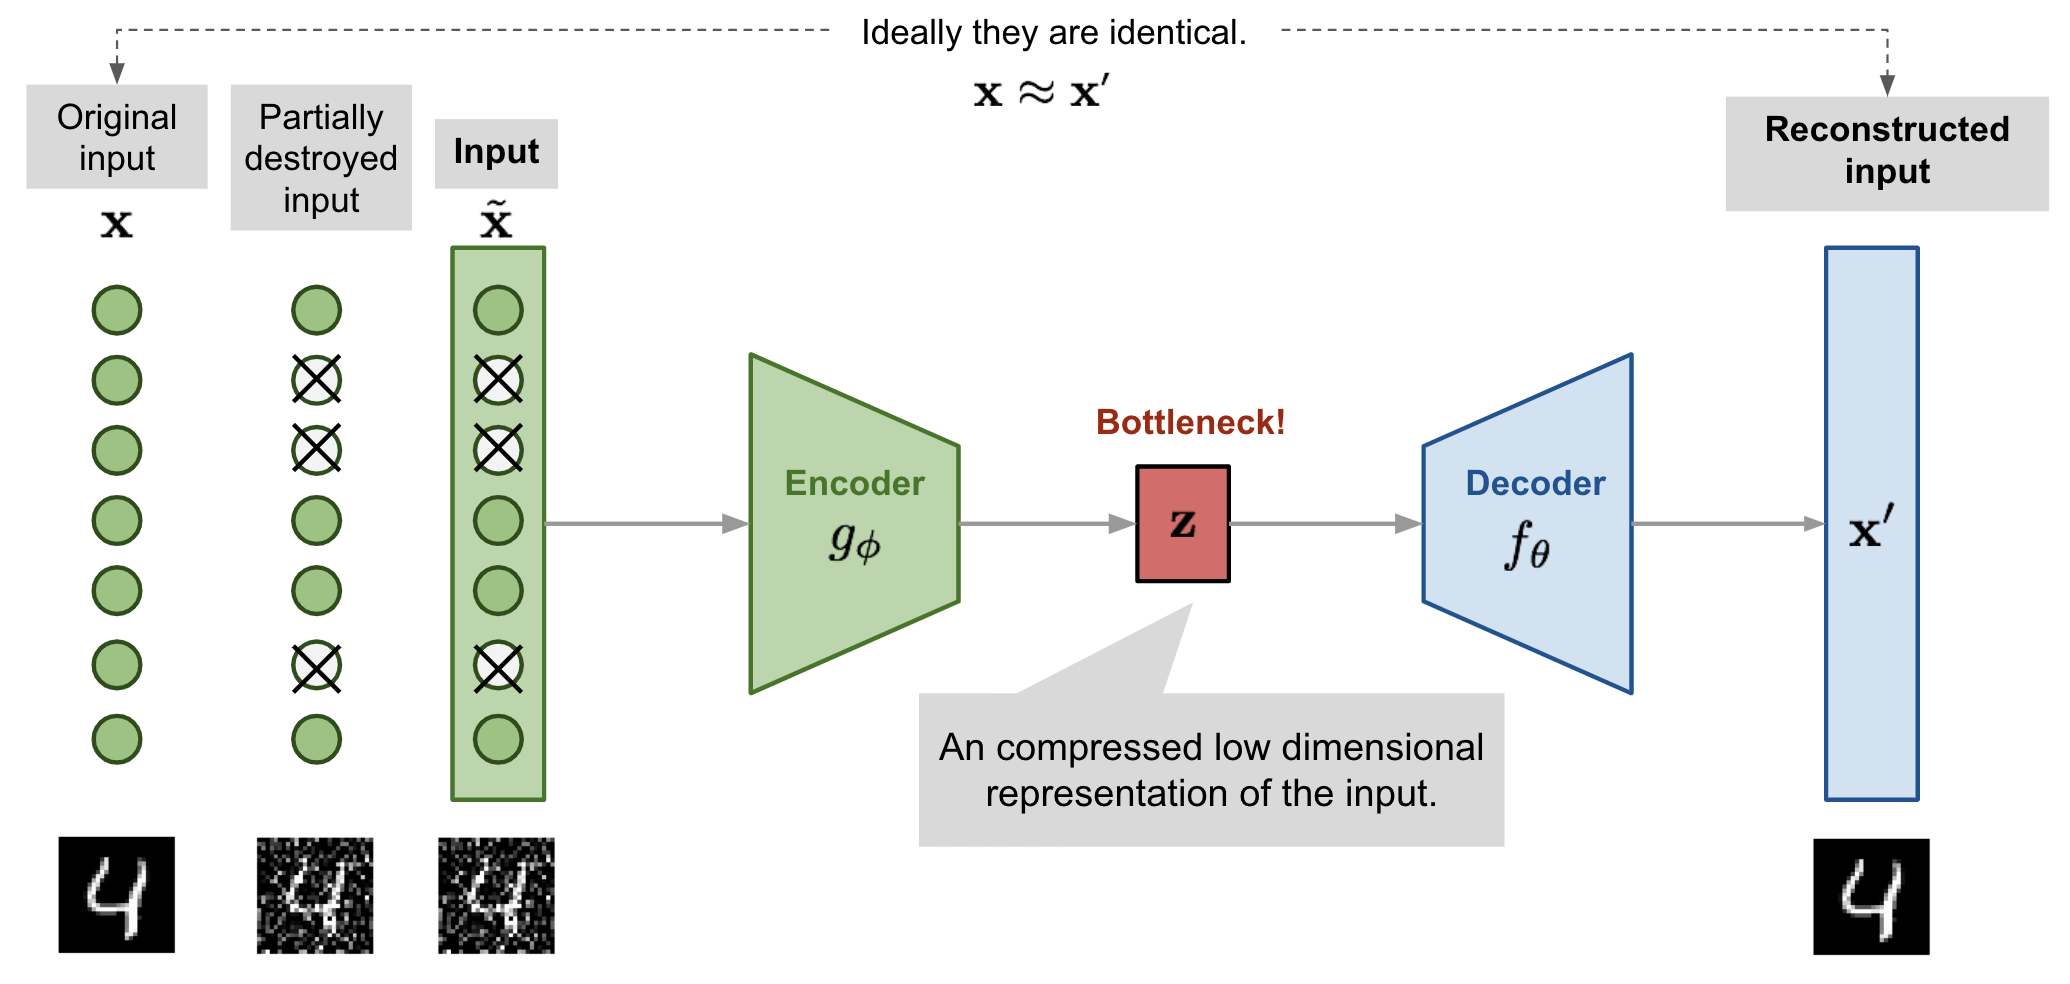
\includegraphics[width=\linewidth]{./images/figures/dae.png}
	\end{center}
	\caption{مدل خود رمز کننده حذف نویز}
	\label{fig:dae}
	\centering
\end{figure}

\section{خودرمزکننده \lr{RDA}}
خودرمزکننده‌هایی که تا کنون معرفی شدند، در مرحله آموزش مدل تنها از دادگان عادی و بدون ناهنجاری استفاده می‌کردند و دادگان ناهنجار تنها زمان آزمون مدل استفاده می‌شدند. حال اگر بخواهیم دادگان ناهنجار را نیز در فرآیند آموزش مدل دخیل کنیم باید روش جدیدی را معرفی کنیم. خودرمز کننده مقاوم\LTRfootnote{Robust Deep AutoEncoder} درواقع از ایده تجزیه و تحلیل مؤلفه بنیادی مقاوم\LTRfootnote{Robust PCA} برگرفته شده است. در روش تجزه و تحلیل مؤلفه 
بنیادی مقاوم، دادگان ورودی با استفاده از دو ماتریس مرتبه پایین\LTRfootnote{Low rank} و خلوت\LTRfootnote{Sparse} نمایش داده می‌شوند.
\begin{equation}
	X = L + S
\end{equation}
که در اینجا $L$ نمایش داده ورودی در ابعاد پایین‌تر است و $S$ قسمتی از دادگان است که نمی‌تواند توسط $L$ به خوبی نمایش داده شود. این دوماتریس تحت شرط بهینه‌سازی و تابع هدف زیر آموزش داده می‌شوند
\footnote{
در اینجا
 $||.||_F$ 
نرم \lr{frobenius} و 
$||.||_*$
 جمع مقادیر یکتا(\lr{singular value}) است.
}
.
\begin{equation}
	||X-L-S||_F^2 = 0
\end{equation}

\begin{equation}
	min_{L,S} ||L||_* + \lambda||S||_1
\end{equation}

این روش نیز سعی دارد دادگان ورودی را به استفاده از دو ماتریس نمایش دهد که ماتریس اول بازنمایی بدست آمده توسط خودرمزکننده است و قسمت دوم نمایانگر ناهنجاری‌هایی است که نمی‌توانند توسط خودرمزکنند به خوبی بازنمایی شوند.
\begin{equation}
X = L_D + S
\end{equation}

اگر رمزکنند و رمزگشا را به عنوان دو تابع $f$ و $g$ در نظر بگیریم، معادل بهینه سازی مدل به صورت زیر خواهد بود.
\begin{equation}
	min_{\theta} || L_D - G_\theta(F_\theta(L_D)) ||_2 + \lambda ||S||_1
\end{equation}
که شرایط زیر باید در فرایند بهینه سازی صدق کند:
\begin{equation}
X-L_D-S=0
\end{equation}

فرایند امتیاز دهی به ناهنجاری در این نوع خودرمز کننده مشابه روش اصلی خواهد بود. در این جا $S$ در واقع همان ناهنجاری‌های موجود در دادگان هستند که پس از تکمیل فرایند آموزش می‌توانیم از آن استفاده کنیم. این روش در مقایسه با روش سنتی در کاربرد تشخیص ناهنجاری حدود 70 درصد بهتر عمل کرده است~\cite{10.1145/3097983.3098052}.



\section{ خود رمز کننده \lr{VAE}}
مشکل که خودرمز کننده‌هایی که تا کنون معرفی کردیم در این است که نگاشت دادگان به فضای باقی‌مانده به صورت قطعی صورت می‌گیرد. یعنی هر نقطه از فضای ورودی به یک مقطه معین از فضای باقی‌مانده نگاشته می‌شود. از طرف دیگر اگر یک نقطه را به صورت تصادفی در فضای باقی‌مانده، مانند 
$z^{'}$
 را در نظر بگیریم، نمی‌توان به طور قطع گفت که این نقطه به کدام دسته از نقاط تعلق خواهد گرفت. در واقع خودرمز کننده‌هایی که تا کنون مطالعه کردیم به خوبی دادگان ورودی را به فضایی با ابعاد دیگر نگاشت میکردند اما در هیچ یک از این روش‌ها ما اختیاری برا کنترل روند و نحوه این نگاشت نداشتیم. انواع مختلف این رمز کننده‌ها نیز بسته به نیاز، نگاشت‌های گوناگونی را در اختیار ما قرار می‌دادند تا مناسب کاربرد انتخاب شده باشند. برای اینکه در طی فرایند یادگیری ما بر روی نحوه نگاش دادگان به فضای باقی‌مانده کنترل داشته باشیم، نوع دیگری از خودرمزکننده‌ها تحت عنوان خودرمز کننده \lr{VAE}\LTRfootnote{Variational AutoEncoder} معرفی شده است~\cite{vae}. در این روش بجای یادگیری نگاشت گسسته و قطعی دادگان به فضای باقیمانده، سعی می‌شود توزیع دادگان در فضای باقیمانده یاد گرفته شود که در این صورت دادگان در این فضا توضیع پیوسته‌ای خواهند داشت و عمل درون‌یابی نقاط در این فضا کار راحت‌تری خواهد بود.\\

در این روش بجای تلاش برای کمینه کردن اختلاف ورودی مدل با خروجی بازسازی شده توسط مدل، سعی می‌شود تا احتمال درستنمایی نهایی\LTRfootnote{Marginal likelihood} حداکثر شود. معادل تابع بهینه سازی این مدل به صورت زیر تعریف می‌شود.
\begin{figure}[!h]
	\begin{center}
		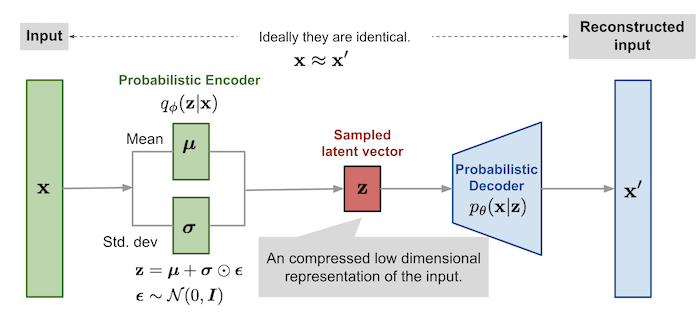
\includegraphics[width=\linewidth]{./images/figures/vae.png}
	\end{center}
	\caption{مدل خود رمز کننده \lr{variational}}
	\label{fig:vae}
	\centering
\end{figure}

\begin{equation}
log(p(x)) \ge log(p(x)) - KL(q_\phi(z|x) || p(z))
\end{equation}

\begin{equation}
log(p(x)) - KL(q_\phi(z|x) || p(z)) = E_{z \sim q_\phi(x)}logP_\phi(x|z)  -  KL(q_\phi(z|x) || p(z))
\end{equation}


\begin{equation}
maximize\  E_{z \sim q_\phi(x)}logP_\phi(x|z)  -  KL(q_\phi(z|x) || p(z))
\label{eq:vae}
\end{equation}

در معادله~\eqref{eq:vae} قسمت اول برای حداکثر کردن احتمال داده باز سازی شده است. قسمت دوم که درواقع می‌توان آن را به عنوان تنظیم کننده معادله درنظر گرفت، تلاش می‌کند تا توزیع دادگان در فضای بازنمایی $z$ بسیار مشابه توزیع دادگان ورودی باشند. بنابراین بازنمایی دادگان در فضای باقیمانده بر خلاف مدل پایه به صورت غیر قطعی\LTRfootnote{Stochastic} خواهد بود. همچنین دادگان بازسازی شده و همچنین امتیاز ناهنجاری برای دادگان نیز غیر قطعی و به صورت احتمال خواهند بود. 


\section{شبکه‌های مولد رقابتی(\lr{GAN})}
شبکه‌های مولد رقابتی\LTRfootnote{Generative Adverserial Networks}از دو قسمت اصلی تشکیل شده‌اند که به صورت رقابتی با یکدیگر آموزش می‌بینند. هر یک از این دو قسمت، سعی دارند عملکرد طرف مقابل را با بالا بردن کیفیت کار خود به چالش بکشند. بخش اول این مدل که مول\LTRfootnote{Generator} نام دارد، مسئولیت تولید داده مصنوعی را بر عهده دارد. این قسمت با گرفتن یک بردار ورودی از فضای باقیمانده، داده‌ای مصنوعی را تولید می‌کند. خروجی این قسمت به همرای یک نمونه از دادگان آموزش برای مقایسه و داوری جهت تشخیص مصنوعی و یا حقیقی بودن به قسمت دوم مدل که تصمیم گیرنده\LTRfootnote{Discriminator} نام دارد وارد می‌شوند. بخش دوم باید بتواند به داده حقیقی که از دادگان آموزش دریافت کرده است برچسب حقیقی و به داده تولید شده توسط بخش مولد برچسب مصنوعی بودن را اختصاص دهد. آموزش این مدل ها به صورت نوبتی صورت می‌گیرد و با شروع از بخش دوم، وزن ها در بخش دیگر ثابت می‌مانند و پس از چند مرحله که عملکرد این قسمت بهبود یافت، تغییر وزن‌ها در آن بخش متوقف شده و وزن‌های بخش دیگر آموزش می‌بینند و پس از بهبود عملکرد قسمت بعدی این چرخه ادامه پیدا می‌کند. تابع خطای مورد استفاده در مدل‌های مولد پایه به صورت زیر است.

\begin{equation}
	min_G max_D V(D, G) = E_{X \sim p_{data}(x)}[logD(x)] + E_{z \sim p_z(z)}[log(1-D(G(z)))]
\end{equation}
برای استفاده از این مدل در تشخیص ناهنجاری‌، استفاده از تابع خطای تصمیم گیرنده به عنوان تابع امتیاز ناهنجاری می‌تواند مفید باشد. در اینصورت، تابع تصمیم گیرنده $D(X)$ وظیفه نگاشت دادگان به فضای تشخیص ناهنجاری را بر عهده دارد و تابع خطای این قسمت از مدل که به صورت زیر تعریف می‌شود به عنوان تابع امتیاز ناهنجاری بکار خواهد رفت.
\begin{equation}
d(x) = log(1- D(X))
\end{equation}
 میزان آستانه تصمیم گیری $\delta$ نیز می‌تواند با استفاده از آزمون و خطا و یا با استفاده از منحنی حساسیت و دقت تعیین گردد.\\


\begin{figure}[!h]
	\begin{center}
		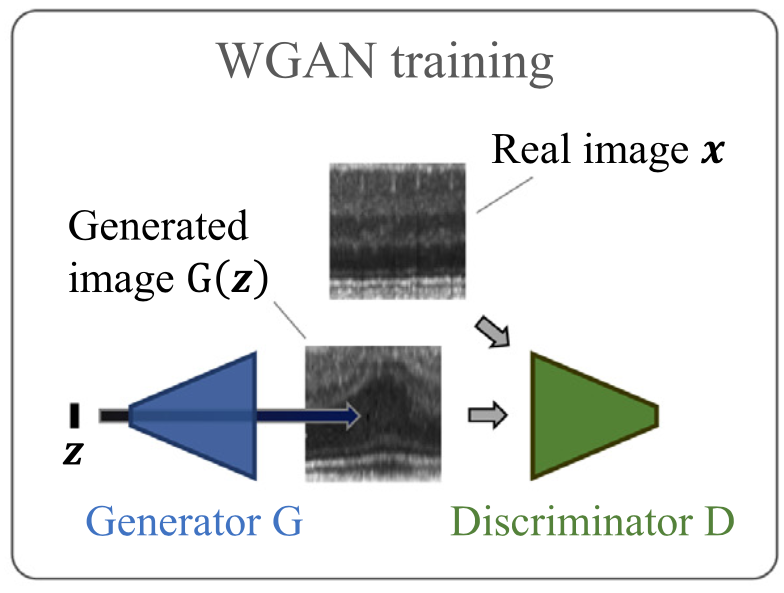
\includegraphics[width=0.7\linewidth]{./images/figures/gan.png}
	\end{center}
	\caption{شبکه مولد رقابتی}
	\label{fig:vae}
	\centering
\end{figure}

برای اینکه بتوانیم از شبکه مولد نیز در این مسئله کمک بگیریم، می‌توانیم در فرایند آموزش دادگان، بجای انتخاب تصادفی یک نقطه از فضای $z$ به عنوان ورودی شبکه مولد، با استفاده از یک رمز کننده دادگان ورودی را ابتدا به رمز کننده بدهیم تا بازنمایی دادگان در فضای باقیمانده بدست آید و سپس این داده را به عنوان ورودی به شبکه مولد بدهیم تا با این بازنمایی اقدام به تولید داده مصنوعی کند. چیزی که در اینجا توقع داریم این است که داده تولید شده توسط تابع مولد، بسیار شبیه به داده ورودی رمز کننده باشد. در این صورت تابع بهینه سازی مدل به صورت زیر خواهد بود.
\begin{equation}
	min_\theta ||G(E(X, \theta)) - X|| + \lambda log(1-D(G(E(X, \theta))))
\end{equation}

در این معادله پارامتر $\lambda$ یک ابر پارامتر مدل است که به صورت دستی تعیین می‌شود. این روش در سال 2017 توسط چلگ و همکاران تحت عنوان \lr{AnoGan} معرفی شد که برای آشکار سازی ناهنجاری‌های در تصاویر  گرفته شده از قرنیه چشم\LTRfootnote{OCT} برای تشخیص بیماری چشم مورد استفاده قرار گرفته است~\cite{10.1007/978-3-319-59050-9_12}. مدل بهبود یافته این روش که با نام \lr{f-AnoGan} توسط همین پژوهشگران معرفی شده است، با جایگذاری روند نگاشت دادگان به فضای باقی‌مانده با یک رمز کننده از پیش آموزش دیده، سرعت محاسبات مدل را بهبود دادند~\cite{SCHLEGL201930}.
\begin{figure}[!h]
	\begin{center}
		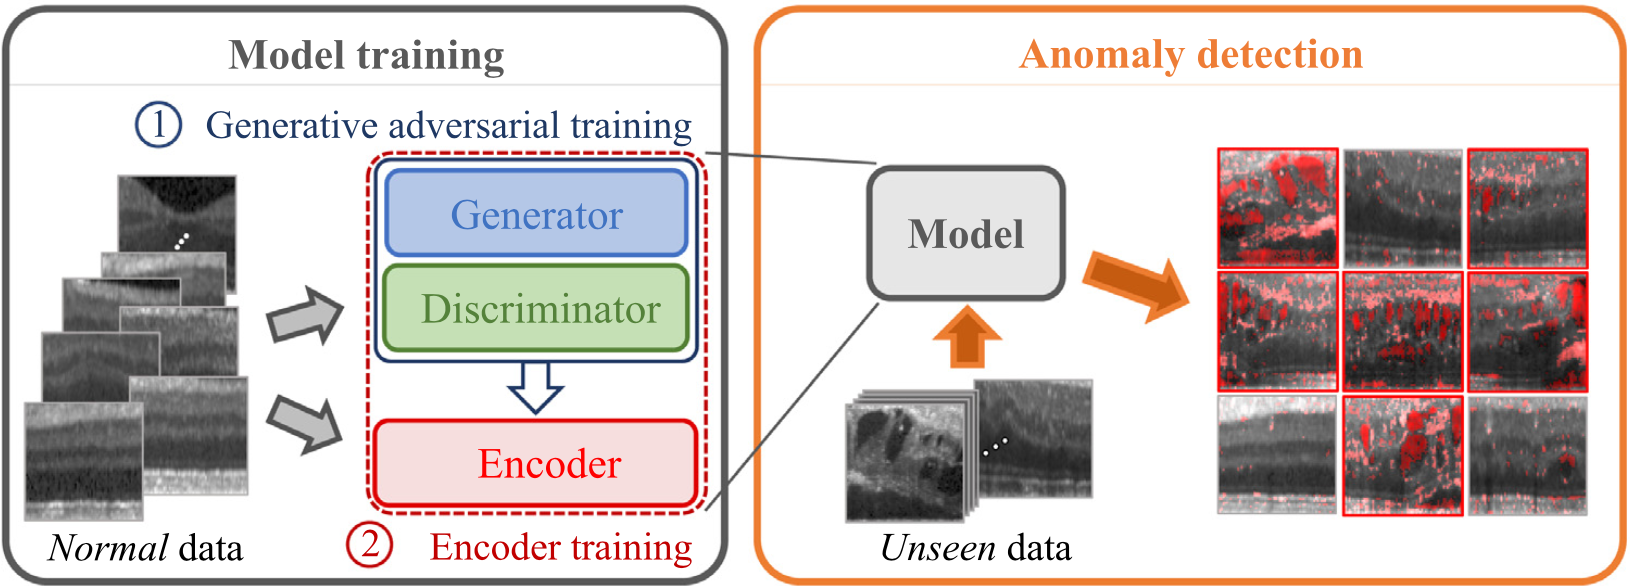
\includegraphics[width=0.7\linewidth]{./images/figures/anogan.png}
	\end{center}
	\caption{نمایش نحوه آموزش مدل \lr{F-AnoGan}~\cite{SCHLEGL201930}}
	\label{fig:vae}
	\centering
\end{figure}

روش دیگری که از رویکرد شبکه‌های مولد استفاده می‌کند، \lr{GANomaly} نام دارد. این روش با هدف تشخیص اشیاء ممنوعه در تصاویر گرفته شده با اشعه ایکس در خطوط کنترل وسایل توسعه داده شده است که عملکرد بهتری نسبت به روش\lr{AnoGan} داشته است~\cite{akcay2018ganomaly}.
\section{مدل‌های جریانی}
مدلهای جریانی\LTRfootnote{Flow based models} مشابه خود رمز کننده \lr{VAE} سعی می‌کنند تا توزیع دادگان ورودی را بیاموزند. در این رویکرد، سعی می‌شود تا با استفاده از یک دنباله از توابع مبدل معکوس پذیر که دادگان را از فضای باقیمانده به فضای ورودی نگاشت می‌کنند، توزیع دادگان آموخته شود. یکی از ایراداتی که بر خودرمز کننده \lr{VAE} در یادگیری توزیع دادگان وارد است، در نظر گرفتن توزیع مانند گوسی برای دادگان است.
\section{بررسی کار‌های انجام شده}
حال که به انواع مختلف روش‌های پایه‌ای آشناشدیم، می‌توانیم به استفاده از این روش‌ها در کاربردهای مختلف بپردازیم. اگر دادگان ما به صورت تصویر، صوت و یا ویدیو باشند، با تغییر لایه‌های کاملا متصل به شبکه‌‌های کانولوشنی می‌توانیم از این معماری برای این کاربرد‌ها استفاده کنیم. همچنین برای دادگان دنباله‌ای مانند متن، سری‌های زمان و غیره نیز میتوانیم با جایگذاری شبکه‌های بازگشتی به جای شبکه کاملا متصل از این روش‌ها استفاده کنیم.

\begin{table}[!h]
	\begin{center}
			\caption{الگوریتم‌های عمیق مورد استفاده در تشخیص ناهنجاری}
			\begin{tabular}{ |c|c|c| } 
				\hline
				\multicolumn{3}{|c|}{روشهای عمیق معروف برای تشخیص ناهنجاری}  \\
				\hline
				
				نام مدل ‌ & مقاله مرجع & ساختار عمیق مورد استفاده \\
				\hline
				\latin{\lr{RDA}} & ژائو و همکاران~\cite{10.1145/3097983.3098052} & خود رمزنگار\\
				\hline
				\latin{\lr{AnoGAN}} & چگل و همکاران~\cite{10.1007/978-3-319-59050-9_12} &شبکه مولد به همراه خود رمزنگار \\
				\hline
				\latin{\lr{f-AnoGan}} & چگل و همکاران~\cite{SCHLEGL201930} & شبکه مولد به همراه خود رمزنگار \\
				\hline
				\latin{\lr{LSA}} & آباتی و همکاران~\cite{abati2019latent} & خود رمزنگار\\
				\hline
				\latin{\lr{ALAD}} & زناتی و همکاران~\cite{Zenati2018AdversariallyLA} & مدل مولد دوجهته\\
				\hline
				\latin{\lr{GANomaly}} & آکای و همکاران~\cite{akcay2018ganomaly} &خودرمزنگار به همراه مدل مولد\\
				\hline
				\latin{\lr{FFP}} & لیو و همکاران~\cite{8578782} & مدل مولد\\
				\hline
				\latin{\lr{EBGAN}} & زناتی و همکاران~\cite{zenati2018} & مدل مولد\\
				\hline
				\latin{\lr{GT}} & گولان و همکاران~\cite{NEURIPS2018_5e62d03a} & استفاده از ساختارهای پایه عمیق\\
				\hline
				\latin{\lr{E3Outlier}} & پانگ و همکاران~\cite{10.1145/3219819.3220042} & استفاده از ساختارهای پایه عمیق\\
				\hline
				\latin{\lr{REPEN}} & ژائو و همکاران~\cite{10.1145/3097983.3098052} & استفاده از ساختارهای پایه عمیق\\
				\hline
				\latin{\lr{RDP}} &وانگ و همکاران~\cite{10.5555/3491440.3491848}& استفاده از ساختارهای پایه عمیق \\
				\hline
				\latin{\lr{AE-OSVM}} & نگویین و همکاران~\cite{Nguyen} & ترکیب خودرمزنگار و روش سنتی\\
				\hline
				\latin{\lr{OC-NN}} & چالاپاتی و همکاران~\cite{chalapathy2018anomaly} & استفاده از ساختارهای پایه عمیق\\
				\hline
				\latin{\lr{Deep SVDD}} & روف و همکاران~\cite{pmlr-v80-ruff18a} & استفاده از ساختارهای پایه عمیق\\
				\hline
				\latin{\lr{Deep SAD}} & روف و همکاران~\cite{ruff2020deep} &  ترکیب خود رمزنگار و روش سنتی\\
				\hline
				\latin{\lr{DAGMM}} & زونگ و همکاران~\cite{Zong2018DeepAG} & استفاده از ساختارهای پایه عمیق\\
				\hline
				\latin{\lr{MIL}} & سلطانی و همکاران~\cite{Sultani_2018_CVPR} & خود رمزنگار\\
				\hline
				\latin{\lr{DevNet}} & پانگ و همکاران~\cite{pang2019deep} & خود رمزنگار\\
				\hline
				\latin{\lr{ALOCC}} & سبکرو و همکاران~\cite{sabokrou2018adversarially} & خود رمزنگار\\
				\hline
				\latin{\lr{OCAN}} & ژنگ و همکاران~\cite{Zheng} & استفاده از ساختارهای پایه عمیق\\
				\hline
				\latin{\lr{FenceGAN}} & ژائو و همکاران~\cite{ngo2019} & شبکه مولد\\
				\hline
				\latin{\lr{OCGAN}} & پررا و همکاران~\cite{8953440} & شبکه مولد\\
				\hline
				\latin{\lr{SPADE}} & کوهن و همکاران~\cite{DBLP:journals/corr/abs-2005-02357} & ساختارهای پایه عمیق\\
				

				\hline
				
				
			
			\end{tabular}

			\label{table:deep-structures}
		\end{center}
\end{table}
	%-------------- Chapter 4--------------
	\chapter{کار‌های آینده}
همانطور که در فصل یک با اهمیت کاربرد روش‌های تشخیص ناهنجاری در حوزه‌های مختلف آشنا شدیم و در فصل دوم و سوم علاوه بر مطالعه روش‌های موجود و مناسب برای مسئله تشخیص ناهنجاری، به بررسی کار‌های انجام شده در این حوزه پرداختیم حال وقت آن رسیده که مسائل و چالش‌های باز این حوزه را مرور کنیم. 
	\section{مسائل باز و کارهای قابل انجام}
در مسائل تشخیص ناهنجاری یکی از چالش‌های مهم، در دسترس نبودن دادگان برچسب خورده کافی و مناسب یادگیری است. با توجه به اینکه ناهنجاری‌ها ذاتا به ندرت اتفاق می‌افتند و همچنین مفهوم ناهنجاری در کاربرد‌های گوناگون متفاوت است، استفاده از روش‌های با ناظر در این مورد مسئله‌ای چالش برانگیز است. یکی از روش‌های پرکاربرد در تشخیص ناهنجاری، یادگیری بازنمایی دادگان عادی است که در فصل سوم به برخی از آنها پرداختیم. در استفاده از این روش‌ها، این احتمال وجود دارد که دادگان آموزش ممکن است دارای خطا باشند که این مورد ممکن است در فرایند یادگیری تاثیر بگذارد. همچنین در بسیاری از کاربرد‌ها مرز مشخص و دقیقی میان دادگان عادی و ناهنجار وجود ندارد. از این رو یافتن روش‌هایی که در مقابل خطا مقاوم باشند یکی از مسائل و چالش‌های بازی در این حوزه است. برای مقابله با چالش کمبود دادگان ناهنجار، ابداع روش‌های داده‌افزایی و بازنمایی دادگان که نیاز به تعداد کمی داده داشته باشند نیز یکی از مسائل باز است. 
	\section{موضوع پیشنهادی برای پایان نامه}
با توجه به کاربرد وسیع مسئله تشخیص ناهنجاری در حوزه پزشکی و مشکل کمبود دادگان برچسب خورده به دلیل چالش‌هایی که در این حوزه وجود دارد، استفاده از روش‌های تشخیص ناهنجاری در این حوزه بسیار مناسب است. در پردازش تصاویر پزشکی به دلیل منحصر به فرد بودن بافت بدن اشخاص مختلف و همچنین نادر بودن بیماری‌ها در میان افراد می‌توان از دید مسئله تشخیص ناهنجاری به وجود توده‌های سرطانی در تصاویر پزشکی نگاه کرد و به بررسی مسئله از این دید پرداخت که می‌تواند به عنوان پیشنهادی برای پروژه پایانی بررسی شود.
	
	
	\newpage
%دستوری برای ظاهر شدن کلمه«مراجع» در فهرست مطالب
\addcontentsline{toc}{section}{مراجع}
%ایجاد «مراجع»
\bibliographystyle{plain-fa}
\bibliography{bibliography.bib}


%\addcontentsline{toc}{section}{نمایه}
%دستوری برای ظاهر شدن کلمه «نمایه» در فهرست مطالب(البته در صورتی که از بسته‌ای که در ابتدا گفته شد استفاده نکرده باشید)
%ایجاد «نمایه»
\printindex
\newpage
\begin{latin}
\chapter*{Abstract}
Anomaly detection is a well studied problem in varios fileds of sciance.
% صفحه آخر ترجمه انگلیسی جلد

\newpage
\thispagestyle{empty}

	\vspace*{25mm}
	\centerline{
\includegraphics[height=4cm]{./images/logos/iust.png}}

	\begin{center}
	\textbf{
Departmant of computer engineering
	}
	\\[1cm]
	\baselineskip=2cm
	{\titr
	\begin{Huge}
	Deep learning for anomaly detection\\[1cm]
	\end{Huge}}
	{\Large 
		\textbf{
			Master seminar report \\
Computer engineering - Artificial intelligence and robotics
		} \\[1cm]
	}

	{\Large { Student name:}
	\\
	{\Large  Ali Naderi Parizi}
	\\[.5cm]
	{\Large  Professor:}
	\\
	{\Large Dr.  Mohsen Soryani}
	\\[.6cm]
	}
April 2022
	\end{center}

\end{latin}
\end{document}
